%
% This is an example LaTeX file which uses the SANDreport class file.
% It shows how a SAND report should be formatted, what sections and
% elements it should contain, and how to use the SANDreport class.
% It uses the LaTeX article class, but not the strict option.
% ItINLreport uses .eps logos and files to show how pdflatex can be used
%
% Get the latest version of the class file and more at
%    http://www.cs.sandia.gov/~rolf/SANDreport
%
% This file and the SANDreport.cls file are based on information
% contained in "Guide to Preparing {SAND} Reports", Sand98-0730, edited
% by Tamara K. Locke, and the newer "Guide to Preparing SAND Reports and
% Other Communication Products", SAND2002-2068P.
% Please send corrections and suggestions for improvements to
% Rolf Riesen, Org. 9223, MS 1110, rolf@cs.sandia.gov
%
\documentclass[pdf,12pt]{INLreport}
% pslatex is really old (1994).  It attempts to merge the times and mathptm packages.
% My opinion is that it produces a really bad looking math font.  So why are we using it?
% If you just want to change the text font, you should just \usepackage{times}.
% \usepackage{pslatex}
\usepackage{times}
\usepackage[FIGBOTCAP,normal,bf,tight]{subfigure}
\usepackage{amsmath}
\usepackage{amssymb}
\usepackage{soul}
\usepackage{pifont}
\usepackage{enumerate}
\usepackage{listings}
\usepackage{fullpage}
\usepackage{xcolor}          % Using xcolor for more robust color specification
\usepackage{ifthen}          % For simple checking in newcommand blocks
\usepackage{textcomp}
\usepackage{mathtools}
\usepackage{relsize}
\usepackage{lscape}
\usepackage[toc,page]{appendix}
\usepackage{RAVEN}

\newtheorem{mydef}{Definition}
\newcommand{\norm}[1]{\lVert#1\rVert}
%\usepackage[table,xcdraw]{xcolor}
%\usepackage{authblk}         % For making the author list look prettier
%\renewcommand\Authsep{,~\,}

% Custom colors
\definecolor{deepblue}{rgb}{0,0,0.5}
\definecolor{deepred}{rgb}{0.6,0,0}
\definecolor{deepgreen}{rgb}{0,0.5,0}
\definecolor{forestgreen}{RGB}{34,139,34}
\definecolor{orangered}{RGB}{239,134,64}
\definecolor{darkblue}{rgb}{0.0,0.0,0.6}
\definecolor{gray}{rgb}{0.4,0.4,0.4}

\lstset {
  basicstyle=\ttfamily,
  frame=single
}


\setcounter{secnumdepth}{5}
\lstdefinestyle{XML} {
    language=XML,
    extendedchars=true,
    breaklines=true,
    breakatwhitespace=true,
%    emph={name,dim,interactive,overwrite},
    emphstyle=\color{red},
    basicstyle=\ttfamily,
%    columns=fullflexible,
    commentstyle=\color{gray}\upshape,
    morestring=[b]",
    morecomment=[s]{<?}{?>},
    morecomment=[s][\color{forestgreen}]{<!--}{-->},
    keywordstyle=\color{cyan},
    stringstyle=\ttfamily\color{black},
    tagstyle=\color{darkblue}\bf\ttfamily,
    morekeywords={name,type},
%    morekeywords={name,attribute,source,variables,version,type,release,x,z,y,xlabel,ylabel,how,text,param1,param2,color,label},
}
\lstset{language=python,upquote=true}

\usepackage{titlesec}
\newcommand{\sectionbreak}{\clearpage}
\setcounter{secnumdepth}{4}

%\titleformat{\paragraph}
%{\normalfont\normalsize\bfseries}{\theparagraph}{1em}{}
%\titlespacing*{\paragraph}
%{0pt}{3.25ex plus 1ex minus .2ex}{1.5ex plus .2ex}

%%%%%%%% Begin comands definition to input python code into document
\usepackage[utf8]{inputenc}

% Default fixed font does not support bold face
\DeclareFixedFont{\ttb}{T1}{txtt}{bx}{n}{9} % for bold
\DeclareFixedFont{\ttm}{T1}{txtt}{m}{n}{9}  % for normal

\usepackage{listings}

% Python style for highlighting
\newcommand\pythonstyle{\lstset{
language=Python,
basicstyle=\ttm,
otherkeywords={self, none, return},             % Add keywords here
keywordstyle=\ttb\color{deepblue},
emph={MyClass,__init__},          % Custom highlighting
emphstyle=\ttb\color{deepred},    % Custom highlighting style
stringstyle=\color{deepgreen},
frame=tb,                         % Any extra options here
showstringspaces=false            %
}}


% Python environment
\lstnewenvironment{python}[1][]
{
\pythonstyle
\lstset{#1}
}
{}

% Python for external files
\newcommand\pythonexternal[2][]{{
\pythonstyle
\lstinputlisting[#1]{#2}}}

\lstnewenvironment{xml}
{}
{}

% Python for inline
\newcommand\pythoninline[1]{{\pythonstyle\lstinline!#1!}}

% Named Colors for the comments below (Attempted to match git symbol colors)
\definecolor{RScolor}{HTML}{8EB361}  % Sonat (adjusted for clarity)
\definecolor{DPMcolor}{HTML}{E28B8D} % Dan
\definecolor{JCcolor}{HTML}{82A8D9}  % Josh (adjusted for clarity)
\definecolor{AAcolor}{HTML}{8D7F44}  % Andrea
\definecolor{CRcolor}{HTML}{AC39CE}  % Cristian
\definecolor{RKcolor}{HTML}{3ECC8D}  % Bob (adjusted for clarity)
\definecolor{DMcolor}{HTML}{276605}  % Diego (adjusted for clarity)
\definecolor{PTcolor}{HTML}{990000}  % Paul

\def\DRAFT{} % Uncomment this if you want to see the notes people have been adding
% Comment command for developers (Should only be used under active development)
\ifdefined\DRAFT
  \newcommand{\nameLabeler}[3]{\textcolor{#2}{[[#1: #3]]}}
\else
  \newcommand{\nameLabeler}[3]{}
\fi
\newcommand{\alfoa}[1] {\nameLabeler{Andrea}{AAcolor}{#1}}
\newcommand{\cristr}[1] {\nameLabeler{Cristian}{CRcolor}{#1}}
\newcommand{\mandd}[1] {\nameLabeler{Diego}{DMcolor}{#1}}
\newcommand{\maljdan}[1] {\nameLabeler{Dan}{DPMcolor}{#1}}
\newcommand{\cogljj}[1] {\nameLabeler{Josh}{JCcolor}{#1}}
\newcommand{\bobk}[1] {\nameLabeler{Bob}{RKcolor}{#1}}
\newcommand{\senrs}[1] {\nameLabeler{Sonat}{RScolor}{#1}}
\newcommand{\talbpaul}[1] {\nameLabeler{Paul}{PTcolor}{#1}}
% Commands for making the LaTeX a bit more uniform and cleaner
\newcommand{\TODO}[1]    {\textcolor{red}{\textit{(#1)}}}
\newcommand{\xmlAttrRequired}[1] {\textcolor{red}{\textbf{\texttt{#1}}}}
\newcommand{\xmlAttr}[1] {\textcolor{cyan}{\textbf{\texttt{#1}}}}
\newcommand{\xmlNodeRequired}[1] {\textcolor{deepblue}{\textbf{\texttt{<#1>}}}}
\newcommand{\xmlNode}[1] {\textcolor{darkblue}{\textbf{\texttt{<#1>}}}}
\newcommand{\xmlString}[1] {\textcolor{black}{\textbf{\texttt{'#1'}}}}
\newcommand{\xmlDesc}[1] {\textbf{\textit{#1}}} % Maybe a misnomer, but I am
                                                % using this to detail the data
                                                % type and necessity of an XML
                                                % node or attribute,
                                                % xmlDesc = XML description
\newcommand{\default}[1]{~\\*\textit{Default: #1}}
\newcommand{\nb} {\textcolor{deepgreen}{\textbf{~Note:}}~}


%%%%%%%% End comands definition to input python code into document

%\usepackage[dvips,light,first,bottomafter]{draftcopy}
%\draftcopyName{Sample, contains no OUO}{70}
%\draftcopyName{Draft}{300}

% The bm package provides \bm for bold math fonts.  Apparently
% \boldsymbol, which I used to always use, is now considered
% obsolete.  Also, \boldsymbol doesn't even seem to work with
% the fonts used in this particular document...
\usepackage{bm}


% Define tensors to be in bold math font.
\newcommand{\tensor}[1]{{\bm{#1}}}

% Override the formatting used by \vec.  Instead of a little arrow
% over the letter, this creates a bold character.
\renewcommand{\vec}{\bm}

% Define unit vector notation.  If you don't override the
% behavior of \vec, you probably want to use the second one.
\newcommand{\unit}[1]{\hat{\bm{#1}}}
% \newcommand{\unit}[1]{\hat{#1}}

% Use this to refer to a single component of a unit vector.
\newcommand{\scalarunit}[1]{\hat{#1}}

% \toprule, \midrule, \bottomrule for tables
\usepackage{booktabs}

% \llbracket, \rrbracket
\usepackage{stmaryrd}

\usepackage{hyperref}
\hypersetup{
    colorlinks,
    citecolor=black,
    filecolor=black,
    linkcolor=black,
    urlcolor=black
}

% Compress lists of citations like [33,34,35,36,37] to [33-37]
\usepackage{cite}

% If you want to relax some of the SAND98-0730 requirements, use the "relax"
% option. It adds spaces and boldface in the table of contents, and does not
% force the page layout sizes.
% e.g. \documentclass[relax,12pt]{SANDreport}
%
% You can also use the "strict" option, which applies even more of the
% SAND98-0730 guidelines. It gets rid of section numbers which are often
% useful; e.g. \documentclass[strict]{SANDreport}

% The INLreport class uses \flushbottom formatting by default (since
% it's intended to be two-sided document).  \flushbottom causes
% additional space to be inserted both before and after paragraphs so
% that no matter how much text is actually available, it fills up the
% page from top to bottom.  My feeling is that \raggedbottom looks much
% better, primarily because most people will view the report
% electronically and not in a two-sided printed format where some argue
% \raggedbottom looks worse.  If we really want to have the original
% behavior, we can comment out this line...
\raggedbottom
\setcounter{secnumdepth}{5} % show 5 levels of subsection
\setcounter{tocdepth}{5} % include 5 levels of subsection in table of contents

% ---------------------------------------------------------------------------- %
%
% Set the title, author, and date
%
\title{RAVEN User Guide}
%\author{%
%\begin{tabular}{c} Author 1 \\ University1 \\ Mail1 \\ \\
%Author 3 \\ University3 \\ Mail3 \end{tabular} \and
%\begin{tabular}{c} Author 2 \\ University2 \\ Mail2 \\ \\
%Author 4 \\ University4 \\ Mail4\\
%\end{tabular} }


\author{
\\Andrea Alfonsi
\\Cristian Rabiti
\\Diego Mandelli
\\Joshua Cogliati
\\Congjian Wang
\\Paul W. Talbot
\\Jia Zhou
\\Pralhad Burli
\\Mohammad G. Abdo
}
%Just people who actually ``developed'' a significant capability in the code should be placed here. Andrea
%\author{\textbf{\textit{Main Developers:}}  \\Andrea Alfonsi}
%\affil{Idaho National Laboratory, Idaho Falls, ID 83402}
%\\\{cristian.rabiti, andrea.alfonsi, joshua.cogliati, diego.mandelli, robert.kinoshita, ramazan.sen\}@inl.gov}

% There is a "Printed" date on the title page of a SAND report, so
% the generic \date should [WorkingDir:]generally be empty.
\date{}


% ---------------------------------------------------------------------------- %
% Set some things we need for SAND reports. These are mandatory
%
\SANDnum{INL/EXT-18-44465}
\SANDprintDate{\today}
\SANDauthor{Andrea Alfonsi, Cristian Rabiti, Diego Mandelli, Joshua Cogliati, Congjian Wang, Paul W. Talbot, Jia Zhou, Pralhad Burli,Mohammad G. Abdo}
\SANDreleaseType{Revision 1}


% ---------------------------------------------------------------------------- %
% Include the markings required for your SAND report. The default is "Unlimited
% Release". You may have to edit the file included here, or create your own
% (see the examples provided).
%
% \include{MarkOUO} % Not needed for unlimted release reports

\def\component#1{\texttt{#1}}

% ---------------------------------------------------------------------------- %
\newcommand{\systemtau}{\tensor{\tau}_{\!\text{SUPG}}}

% Added by Sonat
\usepackage{placeins}
\usepackage{array}

\newcolumntype{L}[1]{>{\raggedright\let\newline\\\arraybackslash\hspace{0pt}}m{#1}}
\newcolumntype{C}[1]{>{\centering\let\newline\\\arraybackslash\hspace{0pt}}m{#1}}
\newcolumntype{R}[1]{>{\raggedleft\let\newline\\\arraybackslash\hspace{0pt}}m{#1}}

% end added by Sonat
% ---------------------------------------------------------------------------- %
%
% Start the document
%

\begin{document}

    \maketitle

    % ------------------------------------------------------------------------ %
    % An Abstract is required for SAND reports
    %
%    \begin{abstract}
%    \input abstract
%    \end{abstract}


    % ------------------------------------------------------------------------ %
    % An Acknowledgement section is optional but important, if someone made
    % contributions or helped beyond the normal part of a work assignment.
    % Use \section* since we don't want it in the table of context
    %
%    \clearpage
%    \section*{Acknowledgment}



%	The format of this report is based on information found
%	in~\cite{Sand98-0730}.


    % ------------------------------------------------------------------------ %
    % The table of contents and list of figures and tables
    % Comment out \listoffigures and \listoftables if there are no
    % figures or tables. Make sure this starts on an odd numbered page
    %
    \cleardoublepage		% TOC needs to start on an odd page
    \tableofcontents
    %\listoffigures
    %\listoftables


    % ---------------------------------------------------------------------- %
    % An optional preface or Foreword
%    \clearpage
%    \section*{Preface}
%    \addcontentsline{toc}{section}{Preface}
%	Although muggles usually have only limited experience with
%	magic, and many even dispute its existence, it is worthwhile
%	to be open minded and explore the possibilities.


    % ---------------------------------------------------------------------- %
    % An optional executive summary
    %\clearpage
    %\section*{Summary}
    %\addcontentsline{toc}{section}{Summary}
    %\input{Summary.tex}
%	Once a certain level of mistrust and skepticism has
%	been overcome, magic finds many uses in todays science



%	and engineering. In this report we explain some of the
%	fundamental spells and instruments of magic and wizardry. We
%	then conclude with a few examples on how they can be used
%	in daily activities at national Laboratories.


    % ---------------------------------------------------------------------- %
    % An optional glossary. We don't want it to be numbered
%    \clearpage
%    \section*{Nomenclature}
%    \addcontentsline{toc}{section}{Nomenclature}
%    \begin{description}
%          \item[alohomoral]
%           spell to open locked doors and containers
%          \item[leviosa]
%           spell to levitate objects
%    \item[remembrall]
%           device to alert you that you have forgotten something
%    \item[wand]
%           device to execute spells
%    \end{description}


    % ---------------------------------------------------------------------- %
    % This is where the body of the report begins; usually with an Introduction
    %
    \SANDmain		% Start the main part of the report

\label{sec:introduction}
RAVEN (Risk Analysis and Virtual control ENviroment), under the support of the Nuclear Energy Advanced Modeling and Simulation (NEAMS) program ~\cite{neams}, is increasing its capabilities to perform probabilistic analysis of stochastic dynamic systems. This supports the goal of providing the tools needed by the Risk Informed Safety Margin Characterization (RISMC) path-lead ~\cite{mandelliANS_RISMC} under the Department of Energy (DOE) Light Water Reactor Sustainability program~\cite{lwrs}. In particular, the development of RAVEN in conjunction with the thermal-hydraulic code RELAP-7~\cite{relap7FY12}, will allow the deployment of advanced methodologies for nuclear power plant (NPP) safety analysis at the industrial level. The investigation of accident scenarios in a probabilistic environment for a complex system (i.e. NPPs) is not a minor task. The complexity of such systems, and a large quantity of stochastic parameters, lead to demanding computational requirements (several CPU/hour). Moreover, high consequence scenarios are usually located in low probability regions of the input space, making even more computational demands of the risk assessment process.

This extreme need for computational power leads to the necessity to investigate methodologies for the most efficient use of available computational resources, either by increasing effectiveness of the global exploration of input space, or by focusing on regions of interest (e.g. failure/success boundaries, etc.). The milestone reported in September 2013 ~\cite{DETmilestone2013} described the capability of RAVEN to perform exploration of the uncertain domain (probabilistic space) through the support of the well-known Dynamic Event Tree (DET) approach. This report will show that the Dynamic Event Tree approach can be considered intrinsically adaptive around the failure prone input zone, if one or more of the uncertain parameters is/are responsible for the transition of interest (e.g. failure or success). Leveraging on this feature is a natural choice to extend the classical DET approach to the Adaptive Dynamic Event Tree (ADET). This extension of the DET methodology to ADET and its implementation in the RAVEN code is the subject of this report. In order to show the effectiveness of this methodology, a Station Black Out (SBO) scenario for a Pressurized Water Reactor has been employed. The ADET approach will be used to focus the exploration of the input space toward the computation of the failure probability of the system (i.e. clad failure). This report is organized in four additional sections. Section 2 recalls the concept of the DET methodology. Section 3 reports how the newer developed algorithm is employed. Section 4 is focused on the analysis performed on the PWR SBO, and, section 5 draws the conclusions.

%\subsection{subsection}
%text

%figure template

%\subsubsection{subsubsection}
%more text
%\paragraph{paragraph}
%lot of text
%\subparagraph{subparagraph}
%if you arrive at this point you have issues

\input{ravenTutorial.tex}
\input{forwardSamplingExample.tex}
\input{adaptiveSamplingExample.tex}
\section{Sampling from Restart}
\label{sec:samplingFromRestart}
In some instances, there are existing solutions stored that are useful to a new sampling calculation.  For
example, if a Monte Carlo run collects 1000 runs, then later the user decides to expand to 1500 runs, the
original 1000 should not be wasted.  In this case, it is desirable to restart sampling.

All \xmlNode{Sampler} entities in RAVEN accept the \xmlNode{Restart} node, which allows the user to provide a
\xmlNode{DataObject} from which sampling can draw.  The way each sampler interacts with this restart data is
dependent on the sampling strategy.

Random sampling strategies, such as the \xmlNode{MonteCarlo} and \xmlNode{Stratified} samplers, increment the
random number generator by the number of samples in the restart data, then continue sampling as normal.

Grid-based sampling strategies, such as \xmlNode{Grid}, \xmlNode{SparseGridCollocation}, and \xmlNode{Sobol},
require specific sampling points.  As each required point in the input space is determined, the sampler will
check the restart data for a match.  If a match is found, the corresponding output values are used instead of
sampling the \xmlNode{Model} for that point in the input space.  In order to determine a match, all of the
values in the restart point must be within a relative tolerance of the corresponding point required by the
sampler.  While RAVEN has a default tolerance of 1e-15, the user can adjust this tolerance using the
\xmlNode{restartNode} node in the \xmlNode{Sampler} block.

In order to demonstrate this restart method, we include here an example of restarting a \xmlNode{Grid}
sampler.  This example runs a simple example Python code from the command line using the \xmlNode{GenericCode}
interface.  Within the run the following steps occur:
\begin{enumerate}
  \item A grid is sampled that includes only the endpoints in each dimension.
  \item The results of the first sampling are written to file.
  \item The results in the CSV are read back in to a new \xmlNode{DataObject} called \xmlString{restart}.
  \item A second, more dense grid is sampled that requires the points of the first sampling, plus several
    more.  The results are added both to the original \xmlNode{DataObject} as well as a new one, for
    demonstration purposes.
  \item The results of only the new sampling can be written to CSV because we added the second data object in
    the last step.
  \item Lastly, the complete \xmlNode{DataObject} is written to file, including both the original and more
    dense sampling.
\end{enumerate}
By looking at the contents of \texttt{GRIDdump1.csv}, \texttt{GRIDdump2.csv}, and \texttt{GRIDdump3.csv}, the
progressive construction of the data object becomes clear.  \texttt{GRIDdump1.csv} contains only a few samples
corresponding to the endpoints of the distributions.  \texttt{GRIDdump3.csv} contains all the points necessary
to include the midpoints of the distributions as well as the endpoints.  \texttt{GRIDdump2.csv} contains only
those points that were not already obtained in the first sampling, but still needed for the more dense
sampling.

\xmlExample[coarse,fine,restart]{framework/Samplers/Restart/Truncated/grid.xml}{Simulation}

In order to restart an existing file that failed for some reason, the
data will need to be listed in the \xmlNode{Files} section and a
\xmlNode{IOStep} that loads that input into a different data object
will be needed to be added to the \xmlNode{Steps} section. After that a \xmlNode{Restart} node can be added.

\xmlExample{framework/Samplers/Restart/test_restart_Grid_part2.xml}{Files}

\xmlExample{framework/Samplers/Restart/test_restart_Grid_part2.xml}{Steps}

\xmlExample{framework/Samplers/Restart/test_restart_Grid_part2.xml}{Samplers}

\section{Reduced Order Modeling through RAVEN}
\label{sec:ROMraven}
The development of high-fidelity codes, for thermal-hydraulic systems
and integrated multi-physics, has undergone a significant acceleration
in the last years. Multi-physics codes simulate
multiple physical models or multiple simultaneous physical phenomena,
in a integrated solving environment. Multi-physics typically
solves coupled systems of partial differential equations, generally
characterized by several different geometrical and time scales.

The new multi-physics codes are characterized by remarkable
improvements
in the approximation of physics (high approximation order and reduced
use of empirical correlations). This greater fidelity is generally
accompanied by a greater computational effort (increased calculation time). This peculiarity is an
obstacle in the application of  computational techniques of
quantification of uncertainty and risk associated with the operation of
particular industrial plant (e.g., a nuclear reactor).

A solution to this problem is represented by the
usage
of highly effective sampling strategies. Sometimes also these
approaches is not enough
in order to perform a comprehensive UQ and PRA analysis. In these
cases the help of reduced order modeling is essential.

RAVEN has support of several different ROMs,
such as:
\begin{enumerate}
  \item \textit{Nearest Neighbors approaches}
  \item \textit{Support Vector Machines}
  \item \textit{Inverse Weight regressors}
  \item \textit{Spline regressors }, etc.
\end{enumerate}

A ROM, also known a surrogate
model, is a mathematical representation of a system, used to predict
a FOM of a physical system.

The ``training'' is a process of setting the internal parameters of the ROM from a set
of samples generated the physical model, i.e.,
 the high-fidelity simulator (RELAP-7, RELAP5
3D, PHISICS, etc.),
\begin{figure}[h!]
  \centering
  \includegraphics[width=1.0\textwidth]  {pics/ROMexampleOfPhysicalSystem.png}
  \caption{Example of reduced order model representation of physical system (regression).}
  \label{fig:ROMexampleOfPhysicalSystem}
\end{figure}

Two characteristics of these models
are generally assumed (even if exceptions are possible):
\begin{enumerate}
  \item The higher the number of realizations in the training sets, the
higher is the accuracy of the prediction performed by the ROM is. This
statement is true for most of the cases, although some ROMs might be
subject to the over-fitting issues. The over-fitting phenomenon is not
analyzed here, since its occurrence highly depends on the
algorithm type, and, hence, the problem needs to be analyzed for all
the large number of ROM types available
  \item The smaller the size of the input (uncertain) domain with
  respect to the variability of the system response, the more likely the
  ROM is able to represent the system response space.
\end{enumerate}

The goals of this section are about learning how to:
 \begin{enumerate}
   \item Set up a sampling strategy to construct multiple ROMs, perturbing a driven code
   \item Train the different ROMs with the data-set obtained by the applied sampling strategy;
   \item Use the same sampling strategy, perturbing the ROMs
   \item Plot the responses of the driven code and ROMs, respectively.
\end{enumerate}
In order to accomplish these tasks, the following RAVEN \textbf{Entities} (XML blocks in the input files) need to be defined:
\begin{enumerate}
   \item \textbf{\textit{RunInfo}}:
     \xmlExample{framework/user_guide/ReducedOrderModeling/reducedOrderModeling.xml}{RunInfo}
   As in the other examples, the \textit{RunInfo} \textbf{Entity} is intended  to set up the analysis sequence that
   needs to be performed. The number of steps specified in (\xmlNode{Sequence}) are sequentially run, eight steps in this specific case, using the number of processors assigned in (\xmlNode{batchSize}).
   \\In the first step, the model is going to be sampled. The obtained results are going to be used to  train three different ROMs.These ROMs are sampled by the same strategy used in the first step in order to compare the ROMs' responses with the ones coming from the original model.
   \item \textbf{\textit{Models}}:
     \xmlExample{framework/user_guide/ReducedOrderModeling/reducedOrderModeling.xml}{Models}
 As mentioned earlier, the goal of this example is the employment of
 a sampling strategy in order to construct multiple types of ROMs.
 \\Indeed, in addition to an External model,
 three different ROMs (GP, SVM and IDW) are here specified. The ROMs will be
 constructed (``trained'') through the data-set generated by the sampling of the External model. Once trained, they are going  to be used in place of the original model.
 \\As it can be seen, the ROMs will be constructed considering two features ($v0,\, and angle,\,$) and two targets  ($r \, and \, t$).
   \item \textbf{\textit{Distributions}}:
     \xmlExample{framework/user_guide/ReducedOrderModeling/reducedOrderModeling.xml}{Distributions}
  In the Distributions XML section, the stochastic model for the
  uncertainties are reported. In
  this case two distributions are defined:
  \begin{itemize}
    \item $vel\_dist \sim \mathbb{N}(30,5)$, used to model the uncertainties
    associated with  the \textit{velocity};
    \item  $angle\_dist \sim \mathbb{U}(5,85)$,  used to
    model the uncertainties associated with the \textit{angle}.
  \end{itemize}
   \item \textbf{\textit{Samplers}}:
     \xmlExample{framework/user_guide/ReducedOrderModeling/reducedOrderModeling.xml}{Samplers}
  To obtain the data-set on which the data mining algorithms are going to be applied, a \textit{MonteCarlo} sampling approach is employed here.
   \item \textbf{\textit{DataObjects}}:
     \xmlExample{framework/user_guide/ReducedOrderModeling/reducedOrderModeling.xml}{DataObjects}
  In this block, six \textit{DataObjects} are defined: 1) PointSet
  named ``samples'' used to collect the final outcomes of the code, 2)
  HistorySet named ``histories'' in which the full time responses of the
  variables are going to be stored, 3) PointSet named
  ``inputPlaceHolder'' used in the \textit{role} of \xmlNode{Input} for the ROMs sampling;
  4) PointSet named ``samplesGP'' used to collect the final outcomes (sampling) of the Gaussian Process (GP) ROM;
  5) PointSet named ``samplesInverse'' used to collect the final outcomes (sampling) of the Inverse Distance Weighting (IDW) ROM;
  6) PointSet named ``samplesSVM'' used to collect the final outcomes (sampling) of the Support Vector Machine (SVM) ROM.
 %%%%%%%%%%%%%%%%%%%%%%%%%%%%%%%%%%%%%%%%%%%%%%%%%%%%%%%%%%
 %%%%%%%%%%%%%%%%%%%%%%%%%%%%%%%%%%%%%%%%%%%%%%%%%%%%%%%%%%
 %figure samples
 \begin{figure}[h!]
  \centering
  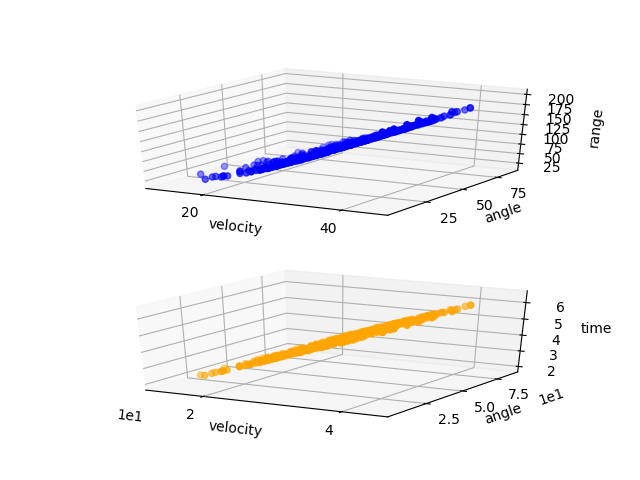
\includegraphics[scale=0.7]{../../tests/framework/user_guide/ReducedOrderModeling/gold/ROMConstruction/1-samplesPlot3D_scatter-scatter.png}
  \caption{Plot of the samples generated by the Monte Carlo sampling}
  \label{fig:ROMgrid_pointsets}
 \end{figure}
 %%%%%%%%%%%%%%%%%%%%%%%%%%%%%%%%%%%%%%%%%%%%%%%%%%%%%%%%%%
 %%%%%%%%%%%%%%%%%%%%%%%%%%%%%%%%%%%%%%%%%%%%%%%%%%%%%%%%%%
   \item \textbf{\textit{OutStreams}}:
     \xmlExample{framework/user_guide/ReducedOrderModeling/reducedOrderModeling.xml}{OutStreams}
     This model makes use of two Print OutStreams and five Plot OutStreams:
     \begin{itemize}
       \item ``samples,'' which writes the contents of the point-wise training samples to CSV,
       \item ``histories,'' which writes the contents of the history-wise training samples to linked CSVs,
       \item ``historyPlot,'' which plots the evolution of the training samples,
       \item ``samplesPlot3D,'' which plots the final state of the training samples with relation to the
         outputs of interest,
       \item ``samplesPlot3DROMgp,'' which plots the validation samples of the Gaussian Process ROM,
       \item ``samplesPlot3DROMsvm,'' which plots the validation samples of the Support-Vector Machine ROM,
       \item ``samplesPlot3Dinverse,'' which plots the validation samples of the multidimensional Inverse
         Weight ROM.
     \end{itemize}
     The 3D plots of the samples as well as the ROM samples can be used as a view-norm validation of the ROMs.
   \item \textbf{\textit{Steps}}:
     \xmlExample{framework/user_guide/ReducedOrderModeling/reducedOrderModeling.xml}{Steps}
  %%%%%%%%%%%%%%%%%%%%%%%%%%%%%%%%%%%%%%%%%%%%%%%%%%%%%%%%%%
 %figure samples
 \begin{figure}[h!]
  \centering
  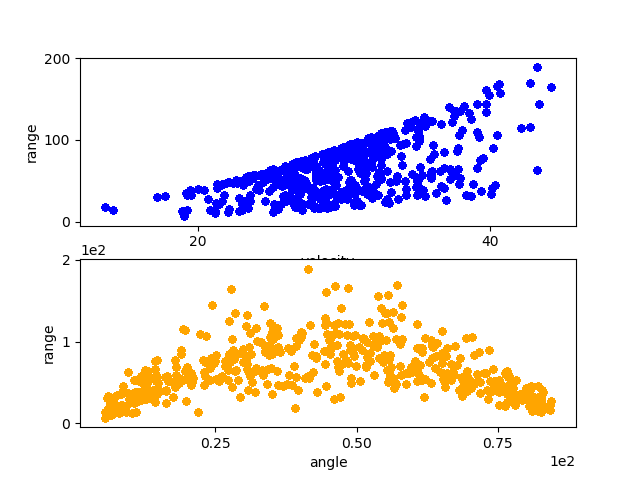
\includegraphics[scale=0.7]{../../tests/framework/user_guide/ReducedOrderModeling/gold/ROMConstruction/1-historyPlot_scatter-scatter.png}
  \caption{Plot of the histories generated by the Monte Carlo method}
  \label{fig:ROMgrid_histories}
 \end{figure}
   %%%%%%%%%%%%%%%%%%%%%%%%%%%%%%%%%%%%%%%%%%%%%%%%%%%%%%%%%%
 %figure samples
 \begin{figure}[h!]
  \centering
  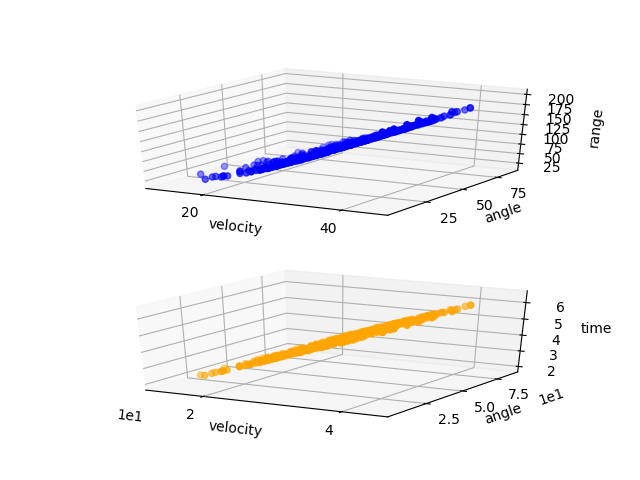
\includegraphics[scale=0.7]{../../tests/framework/user_guide/ReducedOrderModeling/gold/ROMConstruction/1-samplesPlot3DROMgp_scatter-scatter.png}
  \caption{Plot of the samples generated by the Monte Carlo sampling applied on the Gaussian Process ROM}
  \label{fig:ROMgp_samples}
 \end{figure}
 %%%%%%%%%%%%%%%%%%%%%%%%%%%%%%%%%%%%%%%%%%%%%%%%%%%%%%%%%%
 %%%%%%%%%%%%%%%%%%%%%%%%%%%%%%%%%%%%%%%%%%%%%%%%%%%%%%%%%%
   Finally, all the previously defined \textbf{Entities} can be combined in
   the \xmlNode{Steps} block. As inferable,
   eight \xmlNode{Steps} have been inputted:
   \begin{itemize}
     \item \xmlNode{MultiRun} named ``sample'', used to run the multiple
     instances of the driven code and
     collect the outputs in the two \textit{DataObjects}. As it can be
     seen, the \xmlNode{Sampler} is inputted to communicate to the
     \textit{Step} that the driven code needs to
     be perturbed through the Grid sampling strategy;
     \item \xmlNode{RomTrainer} named ``trainROMGaussianProcess'', used to construct (``train'')
     the GP ROM, based on the data-set generated in the  ``sample'' \textbf{Step};
     \item \xmlNode{RomTrainer} named ``trainROMsvm'', used to construct (``train'')
     the SVM ROM, based on the data-set generated in the  ``sample'' \textbf{Step};
     \item \xmlNode{RomTrainer} named ``trainROMinverse'', used to construct (``train'')
     the IDW ROM, based on the data-set generated in the  ``sample'' \textbf{Step};
     \item \xmlNode{MultiRun} named ``sampleROMGaussianProcess'', used to run the multiple
     instances of the previously constructed GP ROM and
     collect the outputs in the PointSet \textit{DataObject}. As it can be
     seen, the same \xmlNode{Sampler} used for perturbing the original model is here used.
     \item \xmlNode{MultiRun} named ``sampleROMsvm'', used to run the multiple
     instances of the previously constructed Support Vector Machine ROM and
     collect the outputs in the PointSet \textit{DataObject}. As it can be
     seen, the same \xmlNode{Sampler} used for perturbing the original model is here used.
     \item \xmlNode{MultiRun} named ``sampleROMInverse'', used to run the multiple
     instances of the previously constructed Inverse Distance Weight ROM and
     collect the outputs in the PointSet \textit{DataObject}. As it can be
     seen, the same \xmlNode{Sampler} used for perturbing the original model is here used.
     \item  \xmlNode{IOStep} named ``writeHistories'', used to 1) export
     the ``histories'' and ``samples''  \textit{DataObjects}
     \textbf{Entity} in a CSV file and 2) plot the responses of the sampling performed on the physical model, GP ROM,
     SVM ROM and IDW ROM in  PNG files and on the screen.
   \end{itemize}
\end{enumerate}

  %figure samples
 \begin{figure}[h!]
  \centering
  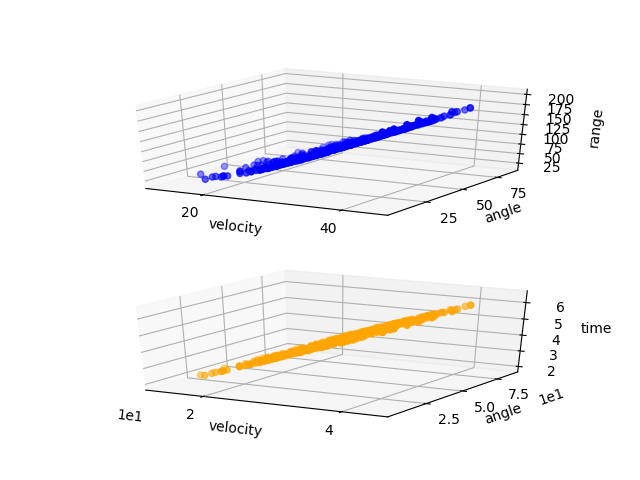
\includegraphics[scale=0.7]{../../tests/framework/user_guide/ReducedOrderModeling/gold/ROMConstruction/1-samplesPlot3DROMsvm_scatter-scatter.png}
  \caption{Plot of the samples generated by the Monte Carlo sampling applied on the Support Vector Machine ROM}
  \label{fig:ROMsvm_samples}
 \end{figure}
 %%%%%%%%%%%%%%%%%%%%%%%%%%%%%%%%%%%%%%%%%%%%%%%%%%%%%%%%%%
  %%%%%%%%%%%%%%%%%%%%%%%%%%%%%%%%%%%%%%%%%%%%%%%%%%%%%%%%%%
  %figure samples
 \begin{figure}[h!]
  \centering
  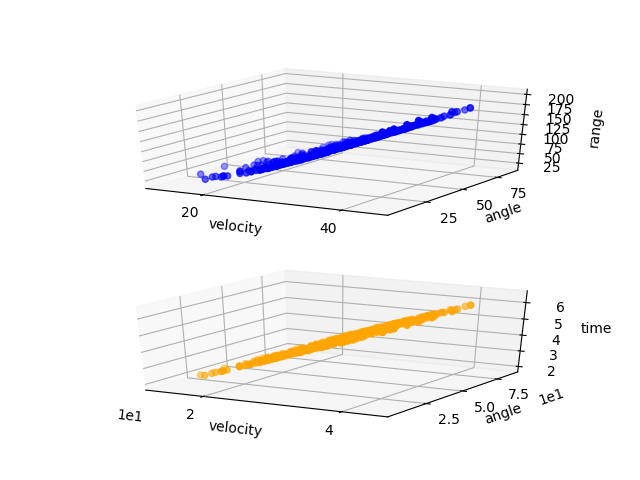
\includegraphics[scale=0.7]{../../tests/framework/user_guide/ReducedOrderModeling/gold/ROMConstruction/1-samplesPlot3DROMinverse_scatter-scatter.png}
  \caption{Plot of the samples generated by the Monte Carlo sampling applied on the Inverse Distance Weight ROM}
  \label{fig:ROMinverse_samples}
 \end{figure}
 %%%%%%%%%%%%%%%%%%%%%%%%%%%%%%%%%%%%%%%%%%%%%%%%%%%%%%%%%%
 Figure \ref{fig:ROMgrid_histories}
 shows the range $r$ for different velocity and angle.
 Figure \ref{fig:ROMgrid_pointsets} shows the final responses  of the sampling employed using the driven code.

Figures \ref{fig:ROMgp_samples}, \ref{fig:ROMsvm_samples} and \ref{fig:ROMinverse_samples}  show the final responses  of the sampling employed using the Gaussian Process, Support Vector Machines and Inverse Distance Weight ROMs, respectively.
It can be clearly noticed that the responses of the ROMs perfectly match the outcomes coming from the original model (see Figure   \ref{fig:ROMgrid_pointsets}).









\section{Statistical Analysis through RAVEN}
\label{sec:SAraven}
In order to perform a complete analysis of a system under uncertainties,
it is crucial to be able to compute all the statistical moments of one or even multiple
FOMs. In addition, it is essential to identify the correlation
among different FOMs toward a specific input space.

RAVEN is able to compute the most important statistical moments:
such as:
\begin{enumerate}
  \item \textit{Expected Value}
  \item \textit{Standard Deviation}
  \item \textit{Variance}
  \item \textit{variationCoefficient}
  \item \textit{Skewness}
  \item \textit{Kurtosis}
  \item \textit{Median}
  \item \textit{Percentile}.
\end{enumerate}
In addition, RAVEN fully supports the computation of all of the statistical moments defined to
``measure'' the correlation among variables/parameters/FOMs:
\begin{enumerate}
  \item \textit{Covariance matrix}
  \item \textit{Normalized Sensitivity matrix}
  \item \textit{Variance Dependent Sensitivity matrix}
  \item \textit{Sensitivity matrix}
  \item \textit{Pearson matrix}.
\end{enumerate}
The goals of this section is to show how to:
 \begin{enumerate}
   \item Set up a sampling strategy to perform a final statistical analysis
   perturbing a driven code
   \item Compute all the statistical moments and correlation/covariance
   metrics.
\end{enumerate}
In order to accomplish these tasks, the following RAVEN \textbf{Entities} (XML blocks in the input files) need to be defined:
\begin{enumerate}
   \item \textbf{\textit{RunInfo}}:
     \xmlExample{framework/user_guide/StatisticalAnalysis/statisticalAnalysis.xml}{RunInfo}
   As shown in the other examples, the \textit{RunInfo} \textbf{Entity} is intended  to set up the desired analysis. The number of steps specified in (\xmlNode{Sequence}) are sequentially run, two steps in this specific case, using the number of processors assigned in (\xmlNode{batchSize}).
   \\In the first step, the original physical model is sampled. The obtained results are  analyzed with the Statistical Post-Processor.
   \item \textbf{\textit{Models}}:
     \xmlExample{framework/user_guide/StatisticalAnalysis/statisticalAnalysis.xml}{Models}
 The goal of this example is to show how the
 principal statistical FOMs can be computed through RAVEN.
 \\We use an External model and specify a Post-Processor model (BasicStatistics). The post-process step is performed on all the output FOMs used in this example ($r and t$).
   \item \textbf{\textit{Distributions}}:
     \xmlExample{framework/user_guide/StatisticalAnalysis/statisticalAnalysis.xml}{Distributions}
  In the Distributions XML section, the stochastic model for the
  uncertainties are reported. In this case 2 distributions are defined:
  \begin{itemize}
    \item $vel\_dist \sim \mathbb{N}(30,5)$, used to model the uncertainties
    associated with  the \textit{velocity};
    \item  $angle\_dist \sim \mathbb{U}(5,85)$,  used to
    model the uncertainties associated with the \textit{angle}.
  \end{itemize}
   \item \textbf{\textit{Samplers}}:
     \xmlExample{framework/user_guide/StatisticalAnalysis/statisticalAnalysis.xml}{Samplers}
  In order to obtain the data-set on which the data mining algorithms are going to be applied, a \textit{MonteCarlo} sampling approach is employed here.
   \item \textbf{\textit{DataObjects}}:
     \xmlExample{framework/user_guide/StatisticalAnalysis/statisticalAnalysis.xml}{DataObjects}
  In this block, three \textit{DataObjects} are defined:
  1) PointSet named ``samples'' used to collect the final outcomes of
  the code,
  2) PointSet named ``dummyIN'' used as a placeholder for the \textit{Multirun} step,
  3) HistorySet named ``histories'' in which the full time responses of the
  variables $x,y,t$ are going to be stored.

   \item \textbf{\textit{Steps}}:
     \xmlExample{framework/user_guide/StatisticalAnalysis/statisticalAnalysis.xml}{Steps}

 %%%%%%%%%%%%%%%%%%%%%%%%%%%%%%%%%%%%%%%%%%%%%%%%%%%%%%%%%%
 %%%%%%%%%%%%%%%%%%%%%%%%%%%%%%%%%%%%%%%%%%%%%%%%%%%%%%%%%%
   Finally, all the previously defined \textbf{Entities} can be combined in
   the \xmlNode{Steps} block. As inferable,
   2 \xmlNode{Steps} have been inputted:
   \begin{itemize}
     \item \xmlNode{MultiRun} named ``sampleMC'', used to run the
     multiple
     instances of the driven code and
     collect the outputs in the two \textit{DataObjects}. As it can be
     seen, the \xmlNode{Sampler} is inputted to communicate to the
     \textit{Step} that the driven code needs to
     be perturbed through the MonteCarlo sampling strategy.
     \item \xmlNode{PostProcess} named ``statisticalAnalysisMC'', used
     compute all the statistical moments and FOMs based on the
     data obtained through the sampling strategy. As it can be noticed,
     the \xmlNode{Output} of the ``sampleMC'' \textit{Step} is the
     \xmlNode{Input} of the ``statisticalAnalysisMC''  \textit{Step}.
   \end{itemize}
\end{enumerate}

Tables \ref{ScalarMoments}-\ref{SensitivityComputed} show all the results of the \textit{PostProcess}
step.


\begin{table}[h!]
\centering
\caption{Computed Moments and Cumulants}
\label{ScalarMoments}
\begin{tabular}{|c|c|c|}
\hline
{\ul \textit{\textbf{Computed Quantities}}} & \textbf{r} & \textbf{t} \\ \hline
\textit{expected value}                     & 65.88   & 3.94   \\ \hline
\textit{median}                             & 61.74   & 4.12   \\ \hline
\textit{variance}                           & 1022.01 & 3.53   \\ \hline
\textit{sigma}                              & 31.97   & 1.89  \\ \hline
\textit{variation coefficient}              & 0.48    & 0.48   \\ \hline
\textit{skewness}                           & 0.55    & -0.03  \\ \hline
\textit{kurtosis}                           & -0.01   & -0.96  \\ \hline
\textit{percentile 5\%}                     & 20.21   & 0.85   \\ \hline
\textit{percentile 95\%}                    & 122.83  & 6.90   \\ \hline
\end{tabular}
\end{table}
\begin{table}[h!]
\centering
\caption{Covariance matrix.}
\label{covarianceComputed}
\begin{tabular}{|c|c|c|}
\hline
{\ul \textit{\textbf{Covariance}}} & \textbf{r} & \textbf{t} \\ \hline
\textit{velocity}                     & 95.36   & 3.29   \\ \hline
\textit{angle}                        & 25.29   & 40.42   \\ \hline
\end{tabular}
\end{table}
\begin{table}[h!]
\centering
\caption{Correlation matrix}
\label{pearsonComputed}
\begin{tabular}{|c|c|c|}
\hline
{\ul \textit{\textbf{Correlation}}} & \textbf{r} & \textbf{t} \\ \hline
\textit{velocity}                     & 0.61   & 0.36   \\ \hline
\textit{angle}                        & 0.03   & 0.92   \\ \hline
\end{tabular}
\end{table}
\begin{table}[h!]
\centering
\caption{Variance Dependent Sensitivity matrix}
\label{VarDepSensitivityComputed}
\begin{tabular}{|c|c|c|}
\hline
{\ul \textit{\textbf{Variance Sensitivity}}} & \textbf{r} & \textbf{t} \\ \hline
\textit{velocity}                     & -1.69   & 0.08   \\ \hline
\textit{angle}                        & -3.31   & 0.07   \\ \hline
\end{tabular}
\end{table}
\begin{table}[h!]
\centering
\caption{Sensitivity matrix}
\label{SensitivityComputed}
\begin{tabular}{|c|c|c|}
\hline
{\ul \textit{\textbf{Sensitivity (I/O)}}} & \textbf{r} & \textbf{t} \\ \hline
\textit{velocity}                     & 3.95   & 0.12   \\ \hline
\textit{angle}                        & 0.01   & 0.07   \\ \hline
\end{tabular}
\end{table}

\subsection{Plotting Multiple Statistical Analyses}
In section \ref{sec:SAraven} we covered how to perform statistical analysis and print the results to an XML
file.  However, what if we want to use the statistics calculated in more RAVEN calculations, like plotting and
further postprocessing?

In the following two sections, we consider two use cases.
\begin{itemize}
  \item In the first case, we want to compare the statistics obtained by three different sampler types on the
    same model. We want to run the sampling, analyze the statistics, then make two plots where we can see how
    the means and variances of the data compare between the sampling strategies.  The plots will have the
    sampler type on the x-axis, and the metric values on the y-axis.
  \item In the second case, we want to see the time evolution of the statistics; that is, the mean and 5/95
    percentile of the model output as it evolves in time.  We want to plot this so that the x-axis is time,
    and the y-axis is the model output value, with three series, one each for fifth percentile, mean, and
    ninety-fifth percentile.
\end{itemize}

Note that while we use the `BasicStatistics` postprocessor as an example, there are many other RAVEN
postprocessors that produce XML outputs that follow this same strategy.

\subsubsection{Case 1: Comparing Samplers}
In this case, we are interested in comparing the statistics obtained by several samplers (Monte Carlo, Grid,
and Stratified/Latin Hypercube) on a plot.  To do
this, we need to complete the following steps:
\begin{enumerate}
  \item Sample the model using Monte Carlo, Grid, and Stratified samplers, storing results in separate point
    sets.
  \item Perform statistical analysis (mean and variance) on each of the point sets containing the samples, writing results to
    separate RAVEN XML output files.
  \item Read in the RAVEN XML output files, creating a point set with the sampler types as inputs and the mean
    and variance as outputs.
  \item Plot the metrics as a function of the sampler used.
\end{enumerate}

These steps lead to the following \xmlNode{RunInfo} block, see especially the \xmlNode{Sequence}:
\xmlExample{framework/user_guide/StatisticalAnalysis/comparingSamplers.xml}{RunInfo}
Note that each sampling and statistics requires its own step, which grows our total steps from four
conceptually to eight in RAVEN.

Next, let's define the \xmlNode{Steps} block that will execute this \xmlNode{sequence}:
\xmlExample{framework/user_guide/StatisticalAnalysis/comparingSamplers.xml}{Steps}

The three ``sample'' steps take the code input (\xmlString{referenceInput}) as input, define the code itself
(\xmlString{bateman}), indicated the sampler to use in each, and then output the results to a
\xmlNode{PointSet}.

The three ``stats'' steps take one of the point sets as input, use the basic statistics postprocessor as the
model, and output to a RAVEN XML output file.  Note that we can re-use a single basic statistics
postprocessor, rather than create separate entities.

In the \xmlString{readStats} step, the three RAVEN XML output files are inputs to the RavenOutput
postprocessor model, and result in a \xmlNode{PointSet} that has the statistics from each file in a single
data object.

In the \xmlString{plot} step, the statistics data object is passed to two \xmlNode{OutStream} plotters.  We
include the \xmlAttr{pauseAtEnd} attribute to ensure plots printed to screen are retained.

With the \xmlNode{Steps} defined, we now define all the entities used throughout the calculation.  We won't go
over them in great detail, but will point out a few notable features:
\begin{itemize}
  \item Data Objects:
    \begin{itemize}
      \item There are three data objects for storing the samples from the samplers, and one to hold the
        statistics.  Note that while the output of the Bateman code is histories, since we only define
        \xmlNode{PointSets} the code keeps only the final value for output values.
    \end{itemize}
  \item Files:
    \begin{itemize}
      \item In order for RAVEN to keep track of the XML files in which the statistics will be written, we
        define them in the \xmlNode{Files} block.  Note that these files need not exist before the RAVEN run
        starts; they will be created in the run.
      \item Additionally, we define the input template for the code itself, used in all the sampling steps.
    \end{itemize}
  \item Models:
    \begin{itemize}
      \item In the Models we define the interface to the Bateman code as well as the two postprocessors.
      \item Note that in the \xmlNode{BasicStatistics} we request the expectedValue, variance, and number of samples as
        metrics for all four outputs of the Bateman model, even though we only need the expectedValue and
        variance for output C.  This demonstrates the ability of the RavenOutput postprocessor to be selective
        about the values it retains.
      \item In the \xmlNode{RavenOutput} postprocessor, there are two operation modes, \xmlNode{dynamic} and
        non-dynamic.  Because the \xmlNode{dynamic} is not specified, we are operating in static mode (we look
        at dynamic mode in the next section).  This means we specify several files to load from.  Ultimately
        we want a point set that contains the following information:
        \begin{center}
        \begin{tabular}{c | c | c }
          ID & mean & variance \\ \hline
          1 & MC mean & MC variance \\
          2 & Grid mean & Grid variance \\
          3 & LHS mean & LHS variance
        \end{tabular}
        \end{center}
        To get these values, we assign a float file ID to each file in the \xmlAttr{ID} attribute.  These
        values can be whatever we want; they'll be used to keep track of which set of outputs come from which
        sampling strategy.  Within the \xmlNode{Files} node, we instruct the RAVEN XML output reader how to
        read in values using the \xmlNode{output} nodes.  The \xmlAttr{name} attribute determines what column
        (or variable) in the PointSet a value will go in, and the text of the node gives a path in the XML to
        find the value.  For example, \xmlString{C|variance} instructs the postprocessor to look in the RAVEN
        XML output file under the node \xmlNode{C} for a node named \xmlNode{expectedValue}, and use its
        value.

        Over the process of reading all the files, entries for both the mean and variance are collected,
        giving us a data set of realizations where the input space is the file ID and the output space are the
        desired metrics.  Note that it is not necessary to retain the original name of the statistics; we
        chose the shorter name ``mean'' to read in the ``expectedValue'' entries.
    \end{itemize}
  \item Samplers and Distributions:
    \begin{itemize}
      \item The Distributions are unchanged from previous examples.
      \item In defining the three samplers, we only note that we specified the number of samples so that they
        were equivalent across all three samplers in an effort to make a fair comparison.
    \end{itemize}
  \item OutStreams:
    \begin{itemize}
      \item We define our two plots here, using fairly standard syntax.  Note that when these plots are
        generated, the File IDs are on the x-axis, while the statistics metric (mean or variance) values are
        on the y-axis.  The File IDs can be traced back to the IDs given in the definition of the
        \xmlNode{RavenOutput} postprocessor.
    \end{itemize}
\end{itemize}
When this code is run, the following plots are produced:
\begin{figure}[h!]
  \centering
  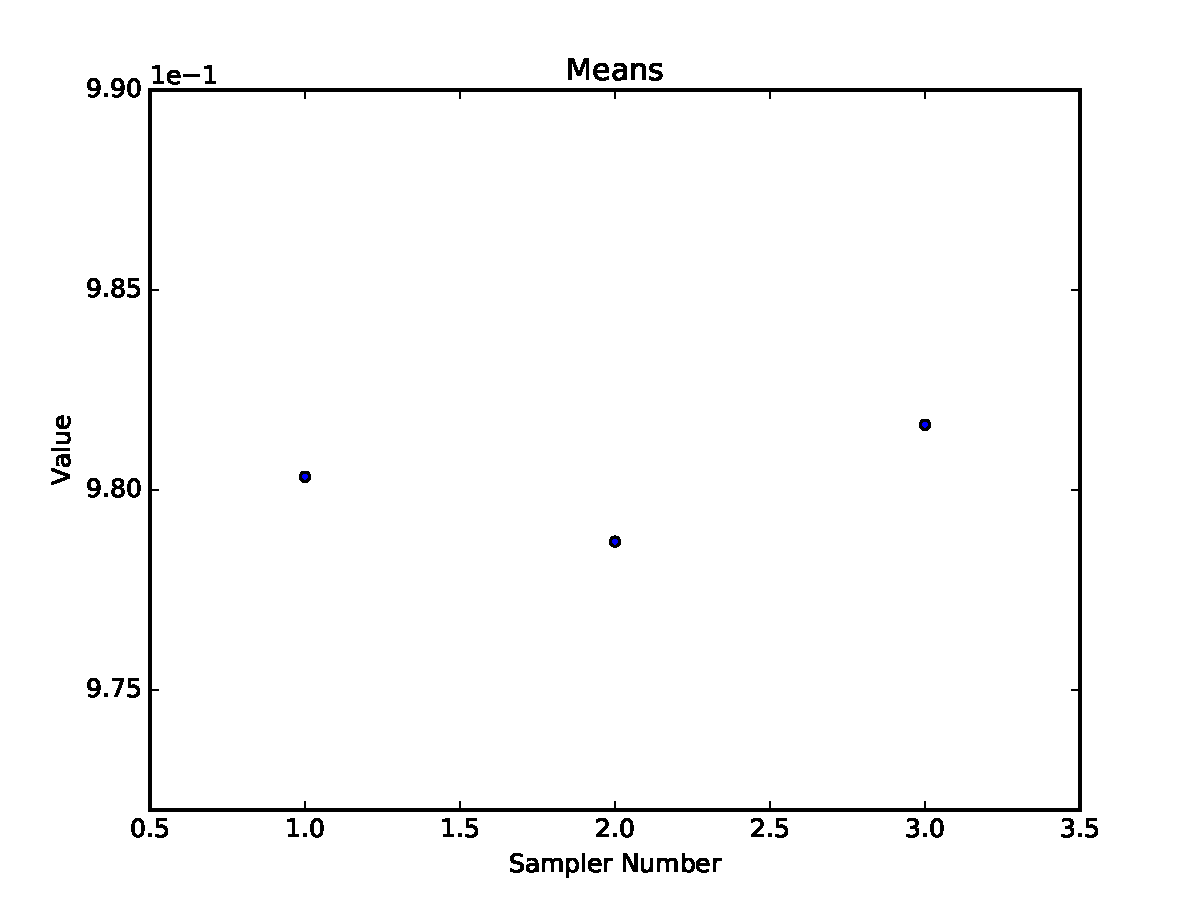
\includegraphics[width=0.7\linewidth]{../../tests/framework/user_guide/StatisticalAnalysis/comparingSamplers/meanPlotter_scatter}
  \caption{Sampler Comparison Plot, Means}
\end{figure}
\begin{figure}[h!]
  \centering
  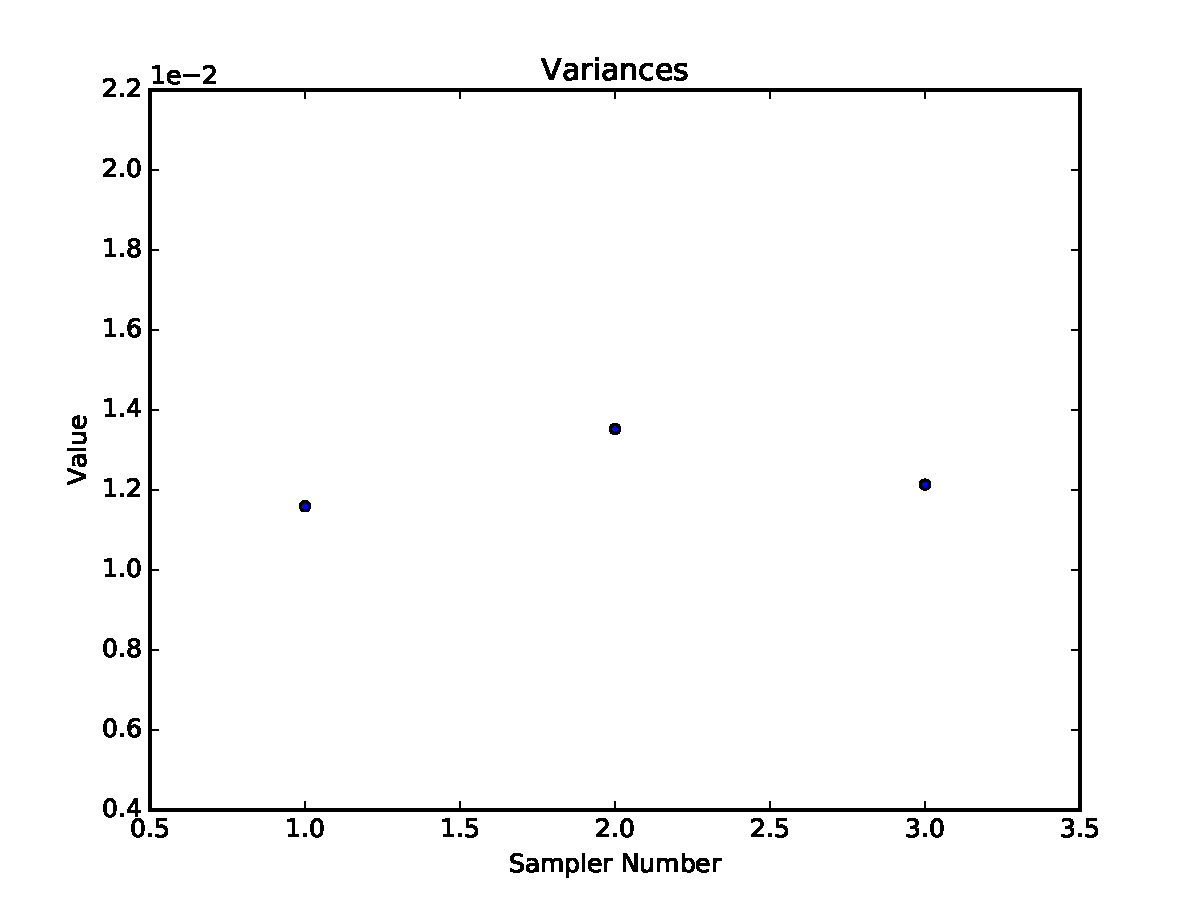
\includegraphics[width=0.7\linewidth]{../../tests/framework/user_guide/StatisticalAnalysis/comparingSamplers/varPlotter_scatter}
  \caption{Sampler Comparison Plot, Variance}
\end{figure}


%%%%%%%%%%%%%%%%%%% OLD
%In order to accomplish these tasks, the following RAVEN \textbf{Entities} need to be defined (these are
%similar to the statistics example in section \ref{sec:SAraven}):
%\begin{enumerate}
%   \item \textbf{\textit{RunInfo}}:
%     \xmlExample{framework/user_guide/StatisticalAnalysis/statisticalAnalysis.xml}{RunInfo}
%   As shown in the other examples, the \textit{RunInfo} \textbf{Entity} is intended  to set up the desired
%   analysis . In this specific case, two steps  (\xmlNode{Sequence}) are sequentially run
%   using forty processors (\xmlNode{batchSize}).
%   \\In the first step, the original physical model is sampled. The obtained results are  analyzed with the
%   Statistical Post-Processor.
%   \item \textbf{\textit{Files}}:
%     \xmlExample{framework/user_guide/StatisticalAnalysis/statisticalAnalysis.xml}{Files}
%   Since the driven code uses a single input file, in this section the original input is placed. As detailed in the user manual
%   the attribute  \xmlAttr{name} represents the alias that is going to be
%   used in all the other input blocks in order to refer to this file.
%   \\In addition, the output file of the \textit{PostProcess} \textbf{Step} is
%   here defined (XML format).
%   \item \textbf{\textit{Models}}:
%     \xmlExample{framework/user_guide/StatisticalAnalysis/statisticalAnalysis.xml}{Models}
% The goal of this example is to show how the
% principal statistical FOMs can be computed through RAVEN.
% \\Indeed, in addition to the previously explained Code
% model, a Post-Processor model (BasicStatistics) is here specified.
%Note that the post-process step is
%performed on all the variables with respect to the parameters used in this example ( $A,\, B,\, C \, and \, D$
%with respect to $sigma-A,\,sigma-B,\, decay-A,$ and $decay-B$).
%   \item \textbf{\textit{Distributions}}:
%     \xmlExample{framework/user_guide/StatisticalAnalysis/statisticalAnalysis.xml}{Distributions}
%  In the Distributions XML section, the stochastic models for the
%  uncertainties are reported. In
%  this case 2 distributions are defined:
%  \begin{itemize}
%    \item $sigma \sim \mathbb{U}(0,1000)$, used to model the uncertainties
%    associated with  the Model \textit{sigma-A} and \textit{sigma-B}
%    \item  $decayConstant \sim \mathbb{U}(1e-8,1e-7)$,  used to
%    model the uncertainties
%    associated with  the Model \textit{decay-A} and \textit{decay-B}.
%  \end{itemize}
%   \item \textbf{\textit{Samplers}}:
%     \xmlExample{framework/user_guide/StatisticalAnalysis/statisticalAnalysis.xml}{Samplers}
%  In order to obtained the data-set through which the statistical FOMs need to be computed, a \textit{MonteCarlo} sampling approach is here employed.
%   \item \textbf{\textit{DataObjects}}:
%     \xmlExample{framework/user_guide/StatisticalAnalysis/statisticalAnalysis.xml}{DataObjects}
%  Int this block, two \textit{DataObjects} are defined:
%  1) PointSet named ``samplesMC'' used to collect the final outcomes of
%  the code,
%  2) HistorySet named ``histories'' in which the full time responses of the
%  variables $A,B,C,D$ are going to be stored.
%
%   \item \textbf{\textit{Steps}}:
%     \xmlExample{framework/user_guide/StatisticalAnalysis/statisticalAnalysis.xml}{Steps}
%
% %%%%%%%%%%%%%%%%%%%%%%%%%%%%%%%%%%%%%%%%%%%%%%%%%%%%%%%%%%
% %%%%%%%%%%%%%%%%%%%%%%%%%%%%%%%%%%%%%%%%%%%%%%%%%%%%%%%%%%
%   Finally, all the previously defined \textbf{Entities} can be combined in
%   the \xmlNode{Steps} block. As inferable,
%   2 \xmlNode{Steps} have been inputted:
%   \begin{itemize}
%     \item \xmlNode{MultiRun} named ``sampleMC'', used to run the
%     multiple
%     instances of the driven code and
%     collect the outputs in the two \textit{DataObjects}. As it can be
%     seen, the \xmlNode{Sampler} is inputted to communicate to the
%     \textit{Step} that the driven code needs to
%     be perturbed through the Grid sampling strategy.
%     \item \xmlNode{PostProcess} named ``statisticalAnalysisMC'', used
%     compute all the statistical moments and FOMs based on the
%     data obtained through the sampling strategy. As it can be noticed,
%     the \xmlNode{Output} of the ``sampleMC'' \textit{Step} is the
%     \xmlNode{Input} of the ``statisticalAnalysisMC''  \textit{Step}.
%   \end{itemize}
%\end{enumerate}
%
%Tables \ref{ScalarMoments}-\ref{SensitivityComputed} show all the results of the \textit{PostProcess}
%step.
%
%
%\begin{landscape}
%\begin{table}[h!]
%\centering
%\caption{Computed Moments and Cumulants.}
%\label{ScalarMoments}
%\begin{tabular}{|c|c|c|c|c|c|c|c|c|}
%\hline
%{\ul \textit{\textbf{Computed Quantities}}} & \textbf{A} & \textbf{B} & \textbf{C} & \textbf{D} & \textbf{decay-A} & \textbf{decay-B} & \textbf{sigma-A} & \textbf{sigma-B} \\ \hline
%\textit{expected value}                     & 5.97E-02   & 3.97E-01   & 9.82E-01   & 1.50E+00   & 5.57E-08         & 5.61E-08         & 5.07E+02         & 4.73E+02         \\ \hline
%\textit{median}                             & 2.45E-02   & 3.06E-01   & 9.89E-01   & 1.54E+00   & 5.73E-08         & 5.62E-08         & 5.11E+02         & 4.70E+02         \\ \hline
%\textit{variance}                           & 8.19E-03   & 6.00E-02   & 1.19E-02   & 1.49E-02   & 7.00E-16         & 6.83E-16         & 8.52E+04         & 8.64E+04         \\ \hline
%\textit{sigma}                              & 9.05E-02   & 2.45E-01   & 1.09E-01   & 1.22E-01   & 2.64E-08         & 2.61E-08         & 2.92E+02         & 2.94E+02         \\ \hline
%\textit{variation coefficient}              & 1.52E+00   & 6.17E-01   & 1.11E-01   & 8.15E-02   & 4.75E-01         & 4.66E-01         & 5.75E-01         & 6.21E-01         \\ \hline
%\textit{skewness}                           & 2.91E+00   & 9.88E-01   & -1.49E-01  & -9.64E-01  & -6.25E-02        & -5.75E-02        & -2.18E-02        & 7.62E-02         \\ \hline
%\textit{kurtosis}                           & 9.56E+00   & -1.12E-01  & -6.98E-01  & -1.50E-01  & -1.24E+00        & -1.21E+00        & -1.21E+00        & -1.20E+00        \\ \hline
%\textit{percentile 5\%}                     & 2.87E-03   & 1.48E-01   & 7.89E-01   & 1.24E+00   & 1.42E-08         & 1.45E-08         & 5.08E+01         & 2.97E+01         \\ \hline
%\textit{percentile 95\%}                    & 2.51E-01   & 9.19E-01   & 1.16E+00   & 1.63E+00   & 9.54E-08         & 9.48E-08         & 9.59E+02         & 9.49E+02         \\ \hline
%\end{tabular}
%\end{table}
%\begin{table}[h!]
%\centering
%\caption{Covariance matrix.}
%\label{covarianceComputed}
%\begin{tabular}{|c|c|c|c|c|c|c|c|c|}
%\hline
%{\ul \textit{\textbf{Covariance}}} & \textbf{A} & \textbf{B} & \textbf{C} & \textbf{D} & \textbf{decay-A} & \textbf{decay-B} & \textbf{sigma-A} & \textbf{sigma-B} \\ \hline
%\textbf{A}                         & 8.19E-03   & -1.11E-03  & -3.09E-03  & -1.13E-04  & -1.28E-09        & 5.14E-11         & -1.49E+01        & -3.74E-01        \\ \hline
%\textbf{B}                         & -1.11E-03  & 6.00E-02   & 2.26E-03   & -2.96E-02  & -7.80E-11        & -6.02E-09        & 7.00E+00         & -1.47E+00        \\ \hline
%\textbf{C}                         & -3.09E-03  & 2.26E-03   & 1.19E-02   & 7.15E-04   & -1.44E-09        & -4.11E-12        & 2.63E+01         & 3.19E-01         \\ \hline
%\textbf{D}                         & -1.13E-04  & -2.96E-02  & 7.15E-04   & 1.49E-02   & -1.21E-10        & 3.01E-09         & 1.12E+00         & 8.01E-01         \\ \hline
%\textbf{decay-A}                   & -1.28E-09  & -7.80E-11  & -1.44E-09  & -1.21E-10  & 7.00E-16         & -1.73E-17        & -1.26E-07        & 2.07E-07         \\ \hline
%\textbf{decay-B}                   & 5.14E-11   & -6.02E-09  & -4.11E-12  & 3.01E-09   & -1.73E-17        & 6.83E-16         & -1.86E-07        & 3.91E-08         \\ \hline
%\textbf{sigma-A}                   & -1.49E+01  & 7.00E+00   & 2.63E+01   & 1.12E+00   & -1.26E-07        & -1.86E-07        & 8.52E+04         & 1.79E+03         \\ \hline
%\textbf{sigma-B}                   & -3.74E-01  & -1.47E+00  & 3.19E-01   & 8.01E-01   & 2.07E-07         & 3.91E-08         & 1.79E+03         & 8.64E+04         \\ \hline
%\end{tabular}
%\end{table}
%\begin{table}[h!]
%\centering
%\caption{Correlation matrix.}
%\label{pearsonComputed}
%\begin{tabular}{|c|c|c|c|c|c|c|c|c|}
%\hline
%{\ul \textit{\textbf{Correlation}}} & \textbf{A} & \textbf{B} & \textbf{C} & \textbf{D} & \textbf{decay-A} & \textbf{decay-B} & \textbf{sigma-A} & \textbf{sigma-B} \\ \hline
%\textbf{A}                          & 1.00E+00   & -5.02E-02  & -3.13E-01  & -1.03E-02  & -5.35E-01        & 2.17E-02         & -5.63E-01        & -1.40E-02        \\ \hline
%\textbf{B}                          & -5.02E-02  & 1.00E+00   & 8.47E-02   & -9.90E-01  & -1.20E-02        & -9.41E-01        & 9.80E-02         & -2.04E-02        \\ \hline
%\textbf{C}                          & -3.13E-01  & 8.47E-02   & 1.00E+00   & 5.37E-02   & -4.98E-01        & -1.44E-03        & 8.25E-01         & 9.96E-03         \\ \hline
%\textbf{D}                          & -1.03E-02  & -9.90E-01  & 5.37E-02   & 1.00E+00   & -3.75E-02        & 9.43E-01         & 3.14E-02         & 2.23E-02         \\ \hline
%\textbf{decay-A}                    & -5.35E-01  & -1.20E-02  & -4.98E-01  & -3.75E-02  & 1.00E+00         & -2.50E-02        & -1.64E-02        & 2.67E-02         \\ \hline
%\textbf{decay-B}                    & 2.17E-02   & -9.41E-01  & -1.44E-03  & 9.43E-01   & -2.50E-02        & 1.00E+00         & -2.44E-02        & 5.08E-03         \\ \hline
%\textbf{sigma-A}                    & -5.63E-01  & 9.80E-02   & 8.25E-01   & 3.14E-02   & -1.64E-02        & -2.44E-02        & 1.00E+00         & 2.08E-02         \\ \hline
%\textbf{sigma-B}                    & -1.40E-02  & -2.04E-02  & 9.96E-03   & 2.23E-02   & 2.67E-02         & 5.08E-03         & 2.08E-02         & 1.00E+00         \\ \hline
%\end{tabular}
%\end{table}
%\begin{table}[h!]
%\centering
%\caption{Variance Dependent Sensitivity matrix.}
%\label{VarDepSensitivityComputed}
%\begin{tabular}{|c|c|c|c|c|c|c|c|c|}
%\hline
%{\ul \textit{\textbf{Variance Sensitivity}}} & \textbf{A} & \textbf{B} & \textbf{C} & \textbf{D} & \textbf{decay-A} & \textbf{decay-B} & \textbf{sigma-A} & \textbf{sigma-B} \\ \hline
%\textbf{A}                                   & 1.00E+00   & -1.36E-01  & -3.77E-01  & -1.38E-02  & -1.56E-07        & 6.27E-09         & -1.82E+03        & -4.56E+01        \\ \hline
%\textbf{B}                                   & -1.86E-02  & 1.00E+00   & 3.77E-02   & -4.94E-01  & -1.30E-09        & -1.00E-07        & 1.17E+02         & -2.45E+01        \\ \hline
%\textbf{C}                                   & -2.60E-01  & 1.90E-01   & 1.00E+00   & 6.01E-02   & -1.21E-07        & -3.46E-10        & 2.21E+03         & 2.68E+01         \\ \hline
%\textbf{D}                                   & -7.60E-03  & -1.99E+00  & 4.80E-02   & 1.00E+00   & -8.11E-09        & 2.02E-07         & 7.51E+01         & 5.37E+01         \\ \hline
%\textbf{decay-A}                             & -1.83E+06  & -1.11E+05  & -2.05E+06  & -1.73E+05  & 1.00E+00         & -2.47E-02        & -1.81E+08        & 2.96E+08         \\ \hline
%\textbf{decay-B}                             & 7.52E+04   & -8.82E+06  & -6.02E+03  & 4.40E+06   & -2.53E-02        & 1.00E+00         & -2.72E+08        & 5.72E+07         \\ \hline
%\textbf{sigma-A}                             & -1.75E-04  & 8.22E-05   & 3.08E-04   & 1.32E-05   & -1.48E-12        & -2.19E-12        & 1.00E+00         & 2.10E-02         \\ \hline
%\textbf{sigma-B}                             & -4.33E-06  & -1.70E-05  & 3.69E-06   & 9.27E-06   & 2.40E-12         & 4.52E-13         & 2.07E-02         & 1.00E+00         \\ \hline
%\end{tabular}
%\end{table}
%\begin{table}[h!]
%\centering
%\caption{Sensitivity matrix.}
%\label{SensitivityComputed}
%\begin{tabular}{|c|c|c|c|c|}
%\hline
%{\ul \textit{\textbf{Sensitivity (I/O)}}} & \textbf{decay-A} & \textbf{decay-B} & \textbf{sigma-A} & \textbf{sigma-B} \\ \hline
%\textbf{A}                                & 3.83E-06         & -1.78E-04        & -2.07E+04        & -1.86E+06        \\ \hline
%\textbf{B}                                & -1.36E-05        & 6.28E-05         & -8.80E+06        & -3.14E+05        \\ \hline
%\textbf{C}                                & 2.17E-06         & 3.05E-04         & 2.64E+04         & -2.00E+06        \\ \hline
%\textbf{D}                                & 6.96E-06         & 2.25E-05         & 4.40E+06         & -6.19E+04        \\ \hline
%\end{tabular}
%\end{table}
%\end{landscape}



\input{dataMiningExample.tex}
\section{Model Optimization}
\label{sec:optimizerStrategies}

When analyzing the range of values obtainable by a model, frequently a key question is ``what set of
parameters result in the best response value?''  To answer this question, RAVEN uses the \xmlNode{Optimizer},
a powerful sampler-like entity that searches the input space to find minimum or maximum values of a response.

In the remainder of this section, we will explore how to use the optimizer using a simple analytic problem,
with a two-dimensional input space and single response of interest.  After getting used to running with the
optimizer, we will add increasing complexity, including changing adaptive step sizes, initial conditions,
parallel trajectories, input space subdivision, input space constraints, and response constraints.

To demonstrate the operation of the Optimizer entities in RAVEN, the model we consider is the Beale function,
which is documented in the analytic tests for RAVEN and replicated here:

\begin{itemize}
  \item Function: $f(x,y) = (1.5-x+xy)^2+(2.25-x+xy^2)^2+(2.625-x+xy^3)^2$
  \item Domain: $-4.5 \leq x,y \leq 4.5$
  \item Global Minimum: $f(3,0.5)=0$
\end{itemize}

The two inputs are the variables $x$ and $y$, and the response is a value we'll assign to $ans$, short for
``answer''.  The model is an external model in RAVEN, and can be found at
\begin{verbatim}
  raven/tests/framework/AnalyticModes/optimizing/beale.py.
\end{verbatim}
The function's values are distributed as in Fig. \ref{fig:beale}, with red indicating high values
and blue indicating low values.
\begin{figure}[h!]
  \centering
  \includegraphics[scale=0.7]{../../tests/framework/user_guide/optimizing/Beale_grid.png}
  \caption{Plot of Beale's function for Optimization}
  \label{fig:beale}
\end{figure}
The objective is to minimize the function.

Note that throughout this example we use the SPSA optimizer by way of demonstration, since it is the first
advanced algorithm for optimization included in RAVEN; many of the options and parameters apply to other
optimizers, and details can be found in the RAVEN user manual.

\subsection{Introduction: The Optimizer Input}
As with other entities, the Optimizer gets its own XML block in the RAVEN input.
Here's an example of an input for a SPSA optimizer named \xmlString{opter}:
\xmlExample{framework/user_guide/optimizing/simple.xml}{Optimizers}
This is the smallest amount of input needed to run an optimization problem, with the exception that we include
the \xmlNode{initialSeed} to maintain consistent results.  Note the required blocks included
to define the optimizer:
\begin{itemize}
  \item \xmlNode{objective}, which is where you indicate the variable for which you want to find the minimum (or,
    if you change the default, maximum).  As listed here, we want to minimize the value of \texttt{ans} given a
    range of possible values for \texttt{x} and \texttt{y}.
  \item \xmlNode{variable}, which is where you can define the input space variables, one for each of these
    nodes.  Declaring a variable here informs the optimizer that you want it to find the optimal value for
    this variable, along with the other variables declared in their own blocks. Note this follows
    the same pattern as any other \xmlNode{Sampler}, including a \xmlNode{distribution} node to
    describe the domain of the variable. For \xmlNode{GradientDescent}, the shape of the
    distribution is not significant unless performing other advanced optimizations (such as
    optimization at risk). Nominally, this distribution simply defines the acceptable range of the
    variable, making the \xmlNode{Uniform} distribution a common choice. The distribution sets the
    upper and lower bounds of the variable, which will give the optimizer some general expectations for
    finding the optimal point; it will never try to sample a value smaller than the lower bound or larger than
    the upper bound.  In the example we define variables \emph{x} and \emph{y} as our input variables, and
    both of them coincidentally range between -4.5 and 4.5.  We set the initial values for both variables to 0
    through the \xmlNode{initial} block, which is required in most cases; the exception is when a
    preconditioner sets them in mulitlevel optimization, but we're not concerned with that feature
    for this example.
  \item \xmlNode{TargetEvaluation}, which declares the DataObject that the optimization search evaluations are
    going to be placed in.  All of the optimal points found as part of the optimization, as well as any other
    points evaluated as part of the algorithm, are placed in this object so the optimizer can retrieve this
    information later.  When this data object is defined, it is critical that the objective variable is
    defined in the output space, and the input variables in the input space, so the optimizer can collect the
    results of its sampling.  The data object type should be ``PointSet'' for this data object.  In this
    example, we use the self-descriptive \emph{optOut} data object.
  \item \xmlNode{samplerInit}, which contains initialization parameters for the optimization
    algorithm. In this case, we set an \xmlNode{initialSeed} to 1234 just to maintain consistent
    results. We also set the maximum number of model evaluations through the \xmlNode{limit} node.
    We don't expect to need all these runs, but in case the optimizer is struggling, we set this
    cutoff to prevent the code running ad infinitum.
  \item \xmlNode{gradient}, which defines the gradient approximation algorithm to use within the
    gradient descent algorithm. In this case,
    we simply indicate that we want to use \xmlNode{SPSA}, and need no additional inputs.
  \item \xmlNode{stepSize}, which defines how we should control the step size during the gradient
    descent algorithm. There are several algorithms to choose from; in this case, we choose
    \xmlNode{GradientHistory}, which uses the scalar product between successive steps to determine
    what step to take in the search algorithm. A bigger growth factor results in traversing the input space more
    quickly, but converging more slowly. A bigger shrink factor results in collapsing to a minimum
    more quickly, converging quickly but possibly falling into local minima. We're using the default
    growth (1.25) and shrink (1.15) factors here.
  \item \xmlNode{acceptance}, which determines the algorithm by which we decide whether to accept a
    potential new optimal point during the gradient descent algorithm. In this case we use
    \xmlNode{Strict}, which indicates any potential new optimal points in the search that are not
    preferrable to the previously-found optimal point are discarded, and the search continues from
    the previously-found optimal point in the search.
  \item \xmlNode{convergence}, which informs the searching algorithm of when to decide it has found
    the optimal point within a sufficient tolerance. There are several stopping criteria; in this
    case, we use the local value of the \xmlNode{gradient}, which we want to be at most 0.1.
\end{itemize}
The other critical blocks in this input are as follows:

\subsubsection{Models}
\xmlExample{framework/user_guide/optimizing/simple.xml}{Models}
Note that we define the external model with the name \xmlString{beale} and provide a path to the analytic
model itself.  This model is set up with the \texttt{run} method that allows RAVEN to run the model.  We also
list all our input/output variables, \emph{x, y}, and \emph{ans}.

\subsubsection{Data Objects}
\xmlExample{framework/user_guide/optimizing/simple.xml}{DataObjects}
We have three data objects:
\begin{itemize}
\item \xmlString{placeholder}, which is necessary to define the input to our external
model in the Steps (the external model doesn't use any input file, so we just use a placeholder
here);
\item \xmlString{optOut}, which will hold all of the samples taken by our optimizer (optimal
candidates, gradient evaluation points, rejected points, etc); and
\item \xmlString{opt\_export}, which will hold the actual solution path taken by our optimizer.  We store the
path travelled by the optimization algorithm as successive samples, with \texttt{iteration} keeping track of the
optimization steps taken.  Note especially how the input of \xmlString{opt\_export} is set to \texttt{trajID},
which is a special keyword for the Optimizer trajectory tracking, as is the output variable \texttt{iteration}.
There are several other special keyword outputs that can be written to the Solution Export data object, that
can be found in the user manual.
\end{itemize}

\subsubsection{Out Streams}
\xmlExample{framework/user_guide/optimizing/simple.xml}{OutStreams}
Here we define the way to print the output of our optimization algorithm.  There's not much to note, except
that we'll be printing the optimization path as a CSV.

\subsubsection{Steps}
\xmlExample{framework/user_guide/optimizing/simple.xml}{Steps}
Here we put it all together into a work flow that RAVEN can follow.  We only need two steps: one to optimize,
and one to print out the results.  To actually perform the optimization, we need a MultiRun step, which we
cleverly name \xmlString{optimize}.  For input we take the placeholder data object \emph{placeholder}, which sets
up the input space of the model we defined, \emph{beal}.  Where a \xmlNode{Sampler} would normally go, we
include the \xmlNode{Optimizer} we defined earlier.  We output to the same data object we indicated in the
Optimizer's \xmlNode{TargetEvaluation} node.  Finally, we note specifically the use of the
\xmlNode{SolutionExport} node.  The data object defined in this node is where the Optimizer will write the
optimization path history, with the final entry being the last step taken by the optimizer.  The IOStep is
unremarkable, used simply to write out the optimization path history to file.

\subsubsection{Conclusion}
After reviewing the components (don't forget the RunInfo block!), you can run this example and see the
results.  In particular, we can view the final results of the optimizer in \texttt{Simple/opt\_export\_0.csv}.  Note
that \texttt{opt\_export} is the name of the \xmlNode{Print} OutStream we defined in the input file.

When we open the file (preferably in a CSV reader such a spreadsheet viewer), we see a CSV with several headers,
the outputs defined in the data object in the input
file: \emph{trajID}, \emph{iteration}, \emph{x}, \emph{y}, and \emph{ans} (not necessarily in that order).  \emph{x},
\emph{y}, and \emph{ans} are the values of the variable at each optimization iteration, while
\emph{iteration} gives the sequential order of the optimization iteration. \emph{trajID} is the
trajectory identifying number; since we are only using one trajectory, this identifier is simply 0.

We can see there's only one line of data in the ouput CSV, showing the final solution discovered by
the optimization algorithm.
If we look at the line, we converged around $f(2.7, 0.42) = 0.0199$ in 40 steps, which is okay but still a little
ways from the analytic optimal point $f(3, 0.5) = 0$.  If we look at the output from the run, we can look at
the last time RAVEN was ``Checking convergence for Trajectory 0''.  Below that statement, there are a series
of convergence criteria and their respeective statuses.  We can see our convergence criteria
requested through the input file (\texttt{gradient}, whose final accepted value is 0.0857) as well
as the \texttt{same point} convergence criteria, which helps determine if the optimal solution is at
a boundary even though other conditions have not converged.

We can see that the reason we converged at the end is the
\texttt{gradient}, which means the relative change in the gradient of \emph{ans} was sufficiently
small between steps to cause convergence.  Clearly, we claimed convergence prematurely because of
the low value required in the optimizer input.  Because these convergence criteria are very
problem-specific, one set parameters will not work best for all problems.

We can improve this result by changing convergence
parameters as well as step size growth and shrink factors, all of which can be found in the user manual, and
many of which we'll discuss in the rest of this section. Feel free to experiment with these values,
and see their affect on the solution discovered.

\subsection{Increasing verbosity}
We saw in the previous section that the output stored in \texttt{Simple/opt\_export.csv} only
includes the final optimal solution, and minimal information about that point. We can increase the
output to see the entire path traversed by adding a few parameters in the input file.

The first parameter to add is in \xmlNode{Optimizers} \xmlNode{GradientDescent}
\xmlNode{samplerInit}. By adding the node \xmlNode{writeSteps} with the value \xmlString{every}, we
can see the full path taken by the optimizer from initial point to final accepted solution.

Further, the optimizer has some special variables that can be use in the \xmlNode{SolutionExport}
\xmlNode{DataObject} to print additional information to the CSV. For example, the special variable
\texttt{accepted} will tell us, for each point in the optimization path, what the result of that
point is. For SPSA, these acceptance notes can be one of the following:
\begin{itemize}
  \item \texttt{first}, or the initial point at which the optimization search begins;
  \item \texttt{accepted}, if the new proposed point is sufficiently improved to be accepted as a
    new optimal point in the search;
  \item \texttt{rejected}, if the new proposed point is \emph{not} sufficiently improved and
    therefore rejected;
  \item \texttt{rerun}, indicating the search algorithm returned to an old optimal point after
    rejecting a proposed optimal point; and
  \item \texttt{final}, which shows that the point listed is the final accepted and converged
    optimal point.
\end{itemize}



\subsection{Initial Conditions and Parallel Trajectories} \label{subsec:opt parallel traj}
Notice we set the optimization search to start at $(0,0)$.
You can change this initial value through
the \xmlNode{initial} block within the \xmlNode{variable} definition nodes.

Furthermore, RAVEN offers the possibility to run multiple optimization paths in parallel.  Because many
(perhaps most) optimization techniques get stuck in local minima, using multiple paths (or \emph{trajectories} as
they are called in RAVEN) increases the likelihood that one of the trajectories will find the global minimum
point.  You can request multiple trajectories by providing a variety of initial conditions in the
\xmlNode{initial} block, as shown in this Optimizer example:
\xmlExample{framework/user_guide/optimizing/multiple_trajectories.xml}{Optimizers}
Note that the ordered pairs are split across the \xmlNode{initial} nodes, so that the first trajectory will
start as a point made up of all the first entries, the second trajectory starts at all the second entries, and
et cetera.  In this case, we've requested starting points at (-2,-2), (-2,2), (2,-2), and (2,2).  This (and
defining a new working directory in the \xmlNode{RunInfo} block) is the only input change between the original
file and this one.

When run, we can see the results in the working directory \texttt{MultipleTraj}.  There, we see the same files
as for the base case, plus \texttt{opt\_export} files 0-3.  These are produced because we've
clustered the outputs by \texttt{trajID} in the \xmlNode{OutStreams} definition. Each of these corresponds to the
path that one of the initial points started at, as you can see at the top of each of these CSV files.  We can
see that trajectory 2 (who started at (2,-2)) ended close to the analytic optimal point, while trajectory 1
was far from it.

In the screen output from the RAVEN run, you can see the final summary shows the status of each
trajectory. Under \emph{Trajectory Results} we see trajectories 1-3 all converged with different
optimal values, while trajectory 0 is marked as \emph{following 1}. This means at some point
Trajectory 0 started following the same path as Trajectory 1 already moved along, so Trajectory 0
was terminated as a result to save computational resources.

Finally, we see the optimal point selected was Trajectory 2 with a function value of roughly 3.7e-3
at (3.15, 0.54).

\subsection{Adjusting Adaptive Steps} \label{subsec:opt stepsize}
As we've seen, some of the optimization paths are struggling to converge to meaningful optimal solutions.
One way to improve this is to tinker with the convergence tolerances as shown in the user manual.  Another is
to change the step size modifications used as part of the search process, which we discuss in this section.
First, we briefly discuss how the SPSA chooses its step size, so we can make informed choices about what
parameters to use.

Because SPSA is a gradient-based method, it operates by starting at a particular point, estimating the
gradient at that point, then taking a step in the opposite direction of the gradient in order to follow a
downhill path.  It adaptively chooses how long of a step to take based on its history.  If the gradient is in
the same direction twice in a row, the algorithm assumes there's further to travel, so increases its step size
multiplicatively by the \emph{growthFactor}, which we had defaulted to 1.25.  If, on the other hand,
the gradient switches directions, then the step size is divided by the \emph{shrinkFactor}, which we
had defaulted to 1.15.  This means that by default, if the gradient keeps going in the same direction, you
always increase your step size by 25\%, while if you're bouncing back and forth in a valley, the
step size is reduced by 15\% at each iteration.

By way of note, in higher dimensions, the actual growth or shrink multiplier is scaled by a dot product
between the two previous gradients, with a max of the grain growth factor when the dot product is 1 (exactly
aligned) and a minimum of grain shrink factor when the dot product is -1 (exactly opposite).  This means if
the gradient is at right angles with the past gradient, then the step size remains unchanged (dot product is
0).

There are some additional considerations for the step size change, as well.  If the algorithm takes a step,
then discovers the new point has a worse response value than the point it's at, it will reject the new point,
re-evaluate the gradient, and flag the step size to be divided by the gain shrink factor.  Because of this, if
the gain shrink factor is too large, false convergence can be obtained when the algorithm struggles to find a
new downhill point to move to.  As a result, in practice it is often beneficial to have a gain shrink factor
that is smaller than the gain growth factor.

For this new example, we use gain growth factor of 1.25 (meaning when the gradient continues in the same
direction our step grows by 25\% of its old value) and a gain shrink factor of 1.1 (meaning when the
gradient flips directions our step size shrinks to 90\% of its old value).  We add this to the base case
(\texttt{simple.xml}) to get:
\xmlExample{framework/user_guide/optimizing/step_size.xml}{Optimizers}
Note the definition of the gain growth and shrink factors in the \xmlNode{convergence} block.  Reviewing the
output file \texttt{StepSize}, we can see more steps were taken than the case using default step sizes, but
the final solution was $f(2.75,0.430)=0.013$ in 40 iterations, which is closer to the analytical solution of $f(3,0.5)=0$
than the original case using the same number of iterations.

It is often challenging to find the best gain growth and shrink factors, and these can have a very significant
impact on the speed and accuracy of the convergence process.  Too large a shrink factor results in poor
resolution of valleys, while too small a shrink factor results in many unnecessary evaluations of the model.

% TODO rewrite with new sampler-based denoising options
% \subsection{Denoising Stochastic Problems}
% While many of the models we see in optimization are deterministic (meaning running the same inputs into the
% model yields the same results every time), there are quite a few stochastic models that we might desire to
% optimize.  For example, a model that included Brownian motion or is solved using unseeded random numbers might
% be considered stochastic.

% The difficulty with optimizing noisy problems rests in the unreliability of a single sample.  If we send a
% single set of inputs into a stochastic model, we can't trust the results to be consistent.  One way to measure
% the consistency of the results is through a signal-to-noise ratio (SNR).  There are many ways to define this
% value; for our purposes, we will use the ratio of the mean of the signal to the standard deviation of the
% signal, $\mu/\sigma$.

% To obtain an approximation of your SNR, you can use RAVEN to perform a Monte Carlo run on your model and then
% use the BasicStatistics postprocessor to collect the mean (expectedValue) and standard deviation (sigma) of
% your response.  It's important to make this sampling all at a single value in the input space, so replace your
% variables with constants in the Sampler input.  Once you have the mean and sigma, you have an idea of how
% noisy your model is.  A SNR of 1 means the signal is just as big as the noise, making it very difficult to
% optimize.  A SNR of less than 1 means the noise dominates the signal, and will make optimization almost
% impossible without introducing denoising.  A SNR of more than 1 indicates the signal is stronger than the
% noise, and perhaps denoising is not necessary.  If your standard deviation is 0, then you don't have any
% discernable noise!

% To denoise a model in RAVEN SPSA optimization currently, we turn our attention to the \xmlNode{Optimizer}
% subnode \xmlNode{parameter}, specifically the \xmlNode{numGradAvgIterations} node.  This parameter instructs
% RAVEN to perform multiple gradient evaluations, including multiple evaluations of each optimal point, and use
% the average to make decisions in optimization pathing.  By default, RAVEN takes one optimal point and one
% neighboring point to evaluate a gradient.  Increasing the \xmlNode{numGradAvgIterations} will increase the
% number of times the optimal point is sampled, and how many neighbor points are sampled.  This serves to
% denoise the model.

% However, this also raises the question, how many resamples do I need to denoise my model?  In a Wilks-like
% approach, we want to reduce the size of the confidence interval for our mean to be less than the noise.  The
% number of resamples required depends on the size of the confidence interval $z$ and the confidence-to-noise ratio
% $\xi$ we want to ultimately have for the optimization algorithm.  We also assume the distribution of the
% response is roughly Gaussian Normal, which may not be the case.  The approximate equation for assuring the
% confidence interval is smaller than the noise is
% \begin{equation}
%   \frac{z\sigma}{\sqrt{n}} \leq \xi\sigma,
% \end{equation}
% \begin{equation}
%   n \geq \left(\frac{z}{\xi}\right)^2.
% \end{equation}
% Thus, the number of resamples depends on the confidence level as well as the desired ratio of the confidence interval
% to the noise.

% A few values for varying ratios are given in Table \ref{tab:confidence levels} for the 99\% confidence level ($z=2.576$).
% \begin{table}[htb]
%   \centering
%   \begin{tabular}{c c}
%     Confidence-to-noise $\xi$ & Resamples necessary \\ \hline
%     1.0 & 7 \\
%     0.9 & 9 \\
%     0.7 & 14 \\
%     0.5 & 27 \\
%     0.1 & 664 \\
%     0.05 & 2655
%   \end{tabular}
%   \caption{Estimate of the number of samples necessary to denoise models to varying confidence levels}
%   \label{tab:confidence levels}
% \end{table}
% That is, if you want the noise and confidence interval to have the same magnitude, only 7 resamples are
% required.  If, on the other hand, you want the confidence interval to be half the level of the noise, 27
% resamples are required.

% Note these are only guidelines; individual models may behave differently and require more or less resamples to
% provide a clear optimization path.

\subsection{Functional Constraints} \label{subsec:opt explicit constraint}
Sometimes an optimization problem has a constrained input space, possibly where there is a tradeoff between
two inputs.  In this event, RAVEN allows the user to define a \emph{constraint} function, which will cause
RAVEN to treat this constraint as it would a boundary condition.

For example, we will introduce a void in the input where we reject inputs.  This void is defined by rejecting
all samples within $(x-1)^2 + y^2 < 1$.  We'll also include the modified step growth and shrink parameters
discussed in section \ref{subsec:opt stepsize}.

To include a constraint function, we first have to define it in the RAVEN input as a \xmlNode{Function}
entity:
\xmlExample{framework/user_guide/optimizing/constrain.xml}{Functions}
Note that the file \texttt{./Constrain/constraint.py} is located relative to the working directory.  Currently,
external functions are always Python files.  In that file,
note that the only method is \texttt{constrain}, which is RAVEN's keyword to find the constraint function.
RAVEN will pass in a \texttt{self} object, which will have the function variables defined in the
\xmlNode{Functions} input available as members.  The method \texttt{constrain} then returns a boolean which is \texttt{True} if
the evaluation does not violate the constraint, or \texttt{False} if the constraint is violated.

To attach the constraint to the optimizer, simply add it as an assembled \xmlNode{Function}:
\xmlExample{framework/user_guide/optimizing/constrain.xml}{Optimizers}

After running, looking through the path followed by trajectory 0 shows that instead of following the path from
section \ref{subsec:opt stepsize}, the path moves to lower \emph{y} values before swinging back up toward the
optimal point.

%\subsection{Implicit Constraints (Penalties)}
% TODO come up with a working example

\input{ensembleModel.tex}
\clearpage
\begin{appendices}
  %
\section{Running RAVEN}
\label{HowToRun}

% I don't think this is mentioned earlier? Andrea answers :D It mentioned in the Introduction
%As already mentioned,
The RAVEN code is a blend of \texttt{C++}, \texttt{C}, and \texttt{Python} languages. The entry point
resides on the \texttt{Python} side and is accessible via a command line interface.
%
After following the instructions in the previous Section, RAVEN is ready to be
used.
%
The RAVEN driver is contained in the folder ``\texttt{raven}.''
%
To run RAVEN, open a terminal and use the following command (replace \texttt{inputFileName.xml} with your RAVEN input file):

\begin{lstlisting}[language=bash]
python raven/raven_framework.py inputFileName.xml
\end{lstlisting}

Alternatively, the \texttt{raven\_framework} script can be used.  In this case, the command is:

\begin{lstlisting}[language=bash]
raven_framework inputFileName.xml
\end{lstlisting}


  \section{Document Version Information}
  \input{../version.tex}
\end{appendices}
%\appendix
\section{Appendix: Example Primer}
\label{sec:examplePrimer}
In this Appendix, a set of examples are reported. In order to be as general as possible, the \textit{Model} type ``ExternalModel'' has been used.
%%%% EXAMPLE 1
\subsection{Example 1.}
\label{subsec:ex1}
This simple example is about the construction of a ``Lorentz attractor'', sampling the relative input space. The parameters that are sampled represent the initial coordinate (x0,y0,z0) of the attractor origin.

\begin{lstlisting}[style=XML,morekeywords={debug,re,seeding,class,subType,limit}]
<?xml version="1.0" encoding="UTF-8"?>
<Simulation verbosity="debug">
<!-- RUNINFO -->
<RunInfo>
    <WorkingDir>externalModel</WorkingDir>
    <Sequence>FirstMRun</Sequence>
    <batchSize>3</batchSize>
</RunInfo>
<!-- Files -->
<Files>
    <Input name='lorentzAttractor.py' type=''>lorentzAttractor</Input>
</Files>
<!-- STEPS -->
<Steps>
    <MultiRun name='FirstMRun'  re-seeding='25061978'>
        <Input   class='Files'     type=''               >lorentzAttractor.py</Input>
        <Model   class='Models'    type='ExternalModel'  >PythonModule</Model>
        <Sampler class='Samplers'  type='MonteCarlo'     >MC_external</Sampler>
        <Output  class='DataObjects'     type='HistorySet'      >testPrintHistorySet</Output>
        <Output  class='Databases' type='HDF5'           >test_external_db</Output>
        <Output  class='OutStreams' type='Print'   >testPrintHistorySet_dump</Output>
    </MultiRun >
</Steps>
<!-- MODELS -->
<Models>
    <ExternalModel name='PythonModule' subType='' ModuleToLoad='externalModel/lorentzAttractor'>
       <variables>sigma,rho,beta,x,y,z,time,x0,y0,z0</variables>
    </ExternalModel>
</Models>
<!-- DISTRIBUTIONS -->
<Distributions>
    <Normal name='x0_distrib'>
        <mean>4</mean>
        <sigma>1</sigma>
    </Normal>
    <Normal name='y0_distrib'>
        <mean>4</mean>
        <sigma>1</sigma>
    </Normal>
    <Normal name='z0_distrib'>
        <mean>4</mean>
        <sigma>1</sigma>
    </Normal>
</Distributions>
<!-- SAMPLERS -->
<Samplers>
    <MonteCarlo name='MC_external'>
      <samplerInit>
        <limit>3</limit>
      </samplerInit>
      <variable name='x0' >
        <distribution  >x0_distrib</distribution>
      </variable>
      <variable name='y0' >
        <distribution  >y0_distrib</distribution>
      </variable>
      <variable name='z0' >
        <distribution  >z0_distrib</distribution>
      </variable>
    </MonteCarlo>
</Samplers>
<!-- DATABASES -->
<Databases>
  <HDF5 name="test_external_db"/>
</Databases>
<!-- OUTSTREAMS -->
<OutStreams>
  <Print name='testPrintHistorySet_dump'>
    <type>csv</type>
    <source>testPrintHistorySet</source>
  </Print>
</OutStreams>
<!-- DATA OBJECTS -->
<DataObjects>
    <HistorySet name='testPrintHistorySet'>
        <Input>x0,y0,z0</Input>
        <Output>time,x,y,z</Output>
   </HistorySet>
</DataObjects>
</Simulation>
\end{lstlisting}
The Python \textit{ExternalModel} is reported below:
\begin{lstlisting}[language=python]
import numpy as np

def run(self,Input):
  max_time = 0.03
  t_step = 0.01

  numberTimeSteps = int(max_time/t_step)

  self.x = np.zeros(numberTimeSteps)
  self.y = np.zeros(numberTimeSteps)
  self.z = np.zeros(numberTimeSteps)
  self.time = np.zeros(numberTimeSteps)

  self.x0 = Input['x0']
  self.y0 = Input['y0']
  self.z0 = Input['z0']

  self.x[0] = Input['x0']
  self.y[0] = Input['y0']
  self.z[0] = Input['z0']
  self.time[0]= 0

  for t in range (numberTimeSteps-1):
    self.time[t+1] = self.time[t] + t_step
    self.x[t+1]    = self.x[t] +  self.sigma*
                      (self.y[t]-self.x[t]) * t_step
    self.y[t+1]    = self.y[t] + (self.x[t]*
                      (self.rho-self.z[t])-self.y[t]) * t_step
    self.z[t+1]    = self.z[t] + (self.x[t]*
                          self.y[t]-self.beta*self.z[t]) * t_step
\end{lstlisting}
%%%% EXAMPLE 2
\subsection{Example 2.}
\label{subsec:ex1}
This example shows a slightly more complicated example, that employs the usage of:
\begin{itemize}
    \item \textit{Samplers:} Grid and Adaptive;
    \item \textit{Models:} External, Reduce Order Models and Post-Processors;
    \item \textit{OutStreams:} Prints and Plots;
    \item \textit{Data Objects:} PointSets;
    \item \textit{Functions:} ExternalFunctions.
\end{itemize}
The goal of this input is to compute the ``SafestPoint''.
It provides the coordinates of the farthest
point from the limit surface that is given as an input.
%
The safest point coordinates are expected values of the coordinates of the
farthest points from the limit surface in the space of the ``controllable''
variables based on the probability distributions of the ``non-controllable''
variables.

The term ``controllable'' identifies those variables that are under control
during the system operation, while the ``non-controllable'' variables are
stochastic parameters affecting the system behavior randomly.

The ``SafestPoint'' post-processor requires the set of points belonging to the
limit surface, which must be given as an input.

\begin{lstlisting}[style=XML,morekeywords={debug,re,seeding,class,subType,limit}]
<Simulation verbosity='debug'>

<!-- RUNINFO -->
<RunInfo>
  <WorkingDir>SafestPointPP</WorkingDir>
  <Sequence>pth1,pth2,pth3,pth4</Sequence>
  <batchSize>50</batchSize>
</RunInfo>

<!-- STEPS -->
<Steps>
  <MultiRun name = 'pth1' pauseAtEnd = 'False'>
    <Sampler  class = 'Samplers'  type = 'Grid'           >grd_vl_ql_smp_dpt</Sampler>
    <Input    class = 'DataObjects'     type = 'PointSet'   >grd_vl_ql_smp_dpt_dt</Input>
    <Model    class = 'Models'    type = 'ExternalModel'  >xtr_mdl</Model>
    <Output   class = 'DataObjects'     type = 'PointSet'   >nt_phy_dpt_dt</Output>
  </MultiRun >

  <MultiRun name = 'pth2' pauseAtEnd = 'True'>
    <Sampler          class = 'Samplers'  type = 'Adaptive'      >dpt_smp</Sampler>
    <Input            class = 'DataObjects'     type = 'PointSet'  >bln_smp_dt</Input>
    <Model            class = 'Models'    type = 'ExternalModel' >xtr_mdl</Model>
    <Output           class = 'DataObjects'     type = 'PointSet'  >nt_phy_dpt_dt</Output>
    <SolutionExport   class = 'DataObjects'     type = 'PointSet'  >lmt_srf_dt</SolutionExport>
  </MultiRun>

  <PostProcess name='pth3' pauseAtEnd = 'False'>
    <Input    class = 'DataObjects'          type = 'PointSet'       >lmt_srf_dt</Input>
    <Model    class = 'Models'         type = 'PostProcessor'  >SP</Model>
    <Output   class = 'DataObjects'          type = 'PointSet'     >sfs_pnt_dt</Output>
  </PostProcess>

  <OutStreamStep name = 'pth4' pauseAtEnd = 'True'>
  	<Input  class = 'DataObjects'            type = 'PointSet'  >lmt_srf_dt</Input>
  	<Output class = 'OutStreams' type = 'Print'         >lmt_srf_dmp</Output>
    <Input  class = 'DataObjects'            type = 'PointSet'  >sfs_pnt_dt</Input>
  	<Output class = 'OutStreams' type = 'Print'         >sfs_pnt_dmp</Output>
  </OutStreamStep>
</Steps>

<!-- DATA OBJECTS -->
<DataObjects>
  <PointSet name = 'grd_vl_ql_smp_dpt_dt'>
    <Input>x1,x2,gammay</Input>
    <Output>OutputPlaceHolder</Output>
  </PointSet>

  <PointSet name = 'nt_phy_dpt_dt'>
    <Input>x1,x2,gammay</Input>
    <Output>g</Output>
  </PointSet>

  <PointSet name = 'bln_smp_dt'>
    <Input>x1,x2,gammay</Input>
    <Output>OutputPlaceHolder</Output>
  </PointSet>

  <PointSet name = 'lmt_srf_dt'>
    <Input>x1,x2,gammay</Input>
    <Output>g_zr</Output>
  </PointSet>

  <PointSet name = 'sfs_pnt_dt'>
    <Input>x1,x2,gammay</Input>
    <Output>p</Output>
  </PointSet>
</DataObjects>

<!-- DISTRIBUTIONS -->
<Distributions>
  <Normal name = 'x1_dst'>
    <upperBound>10</upperBound>
    <lowerBound>-10</lowerBound>
  	<mean>0.5</mean>
    <sigma>0.1</sigma>
  </Normal>

  <Normal name = 'x2_dst'>
    <upperBound>10</upperBound>
    <lowerBound>-10</lowerBound>
    <mean>-0.15</mean>
    <sigma>0.05</sigma>
  </Normal>

  <Normal name = 'gammay_dst'>
    <upperBound>20</upperBound>
    <lowerBound>-20</lowerBound>
    <mean>0</mean>
    <sigma>15</sigma>
  </Normal>
</Distributions>

<!-- SAMPLERS -->
<Samplers>
  <Grid name = 'grd_vl_ql_smp_dpt'>
    <variable name = 'x1' >
      <distribution>x1_dst</distribution>
      <grid type = 'value' construction = 'equal' steps = '10' upperBound = '10'>2</grid>
    </variable>
    <variable name='x2' >
      <distribution>x2_dst</distribution>
      <grid type = 'value' construction = 'equal' steps = '10' upperBound = '10'>2</grid>
    </variable>
    <variable name='gammay' >
      <distribution>gammay_dst</distribution>
      <grid type = 'value' construction = 'equal' steps = '10' lowerBound = '-20'>4</grid>
    </variable>
  </Grid>

  <Adaptive name = 'dpt_smp' verbosity='debug'>
    <ROM              class = 'Models'    type = 'ROM'           >accelerated_ROM</ROM>
    <Function         class = 'Functions' type = 'External'      >g_zr</Function>
    <TargetEvaluation class = 'DataObjects'     type = 'PointSet'  >nt_phy_dpt_dt</TargetEvaluation>
    <Convergence limit = '3000' forceIteration = 'False' weight = 'none' persistence = '5'>1e-2</Convergence>
      <variable name = 'x1'>
        <distribution>x1_dst</distribution>
      </variable>
      <variable name = 'x2'>
        <distribution>x2_dst</distribution>
      </variable>
      <variable name = 'gammay'>
        <distribution>gammay_dst</distribution>
      </variable>
  </Adaptive>
</Samplers>

<!-- MODELS -->
<Models>
  <ExternalModel name = 'xtr_mdl' subType = '' ModuleToLoad = 'SafestPointPP/safest_point_test_xtr_mdl'>
    <variables>x1,x2,gammay,g</variables>
  </ExternalModel>

  <ROM name = 'accelerated_ROM' subType = 'SciKitLearn'>
    <Features>x1,x2,gammay</Features>
    <Target>g_zr</Target>
    <SKLtype>svm|SVC</SKLtype>
    <kernel>rbf</kernel>
    <gamma>10</gamma>
    <tol>1e-5</tol>
    <C>50</C>
  </ROM>

  <PostProcessor name='SP' subType='SafestPoint'>
    <!-- List of Objects (external with respect to this PP) needed by this post-processor -->
    <Distribution     class = 'Distributions'  type = 'Normal'>x1_dst</Distribution>
    <Distribution     class = 'Distributions'  type = 'Normal'>x2_dst</Distribution>
    <Distribution     class = 'Distributions'  type = 'Normal'>gammay_dst</Distribution>
    <!- end of the list -->
    <controllable>
    	<variable name = 'x1'>
    		<distribution>x1_dst</distribution>
    		<grid type = 'value' steps = '20'>1</grid>
    	</variable>
    	<variable name = 'x2'>
    		<distribution>x2_dst</distribution>
    		<grid type = 'value' steps = '20'>1</grid>
    	</variable>
    </controllable>
    <non-controllable>
    	<variable name = 'gammay'>
    		<distribution>gammay_dst</distribution>
    		<grid type = 'value' steps = '20'>2</grid>
    	</variable>
    </non-controllable>
  </PostProcessor>
</Models>

<!-- FUNCTIONS -->
<Functions>
  <External name='g_zr' file='SafestPointPP/safest_point_test_g_zr.py'>
    <variable>g</variable>
  </External>
</Functions>

<!-- OUT-STREAMS -->
<OutStreams>
  <Print name = 'lmt_srf_dmp'>
  	<type>csv</type>
  	<source>lmt_srf_dt</source>
  </Print>

  <Print name = 'sfs_pnt_dmp'>
  	<type>csv</type>
  	<source>sfs_pnt_dt</source>
  </Print>
</OutStreams>

</Simulation>
\end{lstlisting}
The Python \textit{ExternalModel} is reported below:
\begin{lstlisting}[language=python]
def run(self,Input):
  self.g = self.x1+4*self.x2-self.gammay
\end{lstlisting}
The ``Goal Function'',the function that defines the transitions with respect the input space coordinates, is as follows:
\begin{lstlisting}[language=python]
def __residuumSign(self):
  if self.g<0 : return  1
  else        : return -1
\end{lstlisting}

%%%%% EXAMPLE 3
%\subsection{Example3}
%\label{subsec:ex1}
%example 3



    % ---------------------------------------------------------------------- %
    % References
    %
    \clearpage
    % If hyperref is included, then \phantomsection is already defined.
    % If not, we need to define it.
    \providecommand*{\phantomsection}{}
    \phantomsection
    \addcontentsline{toc}{section}{References}
    \bibliographystyle{ieeetr}
    \bibliography{raven_user_guide}


    % ---------------------------------------------------------------------- %
    %

    % \printindex

    %\include{distribution}

\end{document}
